\documentclass[final,5p]{elsarticle}
\usepackage{amsmath,amssymb,amsfonts}
\usepackage{microtype,pifont}
\usepackage{graphicx}
\usepackage[dvipsnames]{xcolor}
\usepackage{tikz}
\usetikzlibrary{arrows.meta,positioning,fit,calc,backgrounds}
\usepackage{pgfplots}
\pgfplotsset{compat=1.17}
\usepackage{booktabs,multirow,tabularx,array,makecell}
\usepackage{algorithm,algorithmicx,algpseudocode}
\usepackage{enumitem, float,placeins}
\usepackage{caption}
\usepackage[colorlinks,bookmarksopen,bookmarksnumbered,citecolor=blue, colorlinks=true,linkcolor=blue,urlcolor=blue,breaklinks=true]{hyperref}
\usepackage{xurl}
\usepackage{orcidlink}
\usepackage{balance}
\setlength{\emergencystretch}{3em}
\Urlmuskip=0mu plus 1mu

% =========================
% Commands and styles
% =========================
\newcommand{\cmark}{\textcolor{ForestGreen}{\ding{51}}}
\newcommand{\xmark}{\textcolor{BrickRed}{\ding{55}}}

% --- Revision markers -------------------------------------------------
% \red{...}  : text that depends on experiments still to be run (see todo.md)
% \tbd       : a single number/entry to be filled from new experiments
% Remove or neutralise these macros before submission.
\newcommand{\red}[1]{\textcolor{red}{#1}}
\newcommand{\tbd}{\textcolor{red}{TBD}}
% -----------------------------------------------------------------------

\newcolumntype{R}[1]{>{\raggedleft\arraybackslash}m{#1}}
\newcolumntype{L}[1]{>{\raggedright\arraybackslash}m{#1}}
\newcolumntype{C}[1]{>{\centering\arraybackslash}m{#1}}

\renewcommand{\algorithmicrequire}{\textbf{Input:}}
\renewcommand{\algorithmicensure}{\textbf{Output:}}
\algrenewcommand\algorithmiccomment[1]{\hfill{\footnotesize$\triangleright$ #1}}

\newtheorem{proposition}{Proposition}
\newtheorem{lemma}{Lemma}
\newdefinition{definition}{Definition}
\newproof{proof}{Proof}

\makeatletter
\newcommand{\algorithmautorefname}{Algorithm}
\renewcommand{\figureautorefname}{Figure}
\renewcommand{\tableautorefname}{Table}
\renewcommand{\equationautorefname}{Eq.}
\makeatother

\journal{Computer Networks}

\begin{document}

\begin{frontmatter}

\title{BIZM: Verification-Guided LLM Response Synthesis for Bounded East-West Threat Containment in Zero-Trust Microsegmentation}

\author{Hanh P. Du\orcidlink{0000-0002-8993-1164}}
\ead{hanhdp@vnu.edu.vn}

\author{Hung K. Luu\orcidlink{0009-0006-5229-4858}}
\ead{22024546@vnu.edu.vn}

\author{Minh T. Nguyen\orcidlink{0009-0002-3612-7292}}
\ead{23020628@vnu.edu.vn}

\author{Hoa N. Nguyen\orcidlink{0000-0002-2565-281X}\corref{cor1}}
\ead{hoa.nguyen@vnu.edu.vn}

\cortext[cor1]{Corresponding author}

\affiliation{
    organization={Department of Information Systems, VNU University of Engineering and Technology},
    city={Hanoi},
    postcode={100000},
    country={Vietnam}
}

\begin{abstract}
Zero Trust microsegmentation limits lateral movement in data centers, yet deployed policies are static and cannot respond when a compromised workload abuses a permitted path. Runtime response is usually delegated to SOAR playbooks or, more recently, to LLM agents: playbooks are brittle under unknown signatures, hand-written response rules drift from the architecture they encode, and an LLM on the enforcement path may hallucinate or follow instructions injected into alert text. This paper presents \textbf{BIZM} (\textbf{B}ounded-\textbf{I}solation \textbf{Z}ero-Trust \textbf{M}icrosegmentation), which treats east-west response as a program-synthesis problem under explicit safety invariants. Ahead of time, an LLM synthesizes a response program from the data-center knowledge base in a target-free response language; an exhaustive verifier checks the bounded-isolation invariants on every point of the finite alert domain and returns counterexamples that guide repair; and a majority ensemble of verified programs is deployed and activated only for the knowledge base it was synthesized from. The program answers covered alerts without a model call and abstains otherwise; at runtime, an LLM agent reasons only over the residual alerts. On both paths, deterministic validation and command-level Zero Trust enforcement admit only source-faithful, time-bounded, DROP-only actions, so a wrong or manipulated model cannot widen its authority over the fabric. Experiments on a SONiC spine-leaf testbed with Suricata monitoring show that the synthesized program agrees with the knowledge base on all 14,970 graded points of the alert domain, whereas a hand-written contextual rule reaches 96.1\%; that the verifier rejected three of the six initially synthesized programs, which counterexample-guided repair corrected within one round; and that resynthesis keeps agreement at 99.97\% to 100\% after four knowledge-base changes. On live traffic, BIZM contains all threats without false positives, reduces median decision latency from 3.1 to 0.6 seconds, and produces no unsafe enforcement under the tested adversarial alerts.
\end{abstract}

%% Research highlights (Computer Networks requires 3-5 bullets, max 85 characters each, submitted as a separate file).
%% \begin{highlights}
%% \item East-west response is cast as program synthesis under bounded-isolation invariants.
%% \item An LLM synthesizes a response program; an exhaustive verifier guides its repair.
%% \item The verified program agrees with the knowledge base on all 14,970 graded alerts.
%% \item Fail-closed validation and DROP-only enforcement bound a wrong or injected model.
%% \item Live containment on a SONiC testbed cuts decision latency from 3.1 s to 0.6 s.
%% \end{highlights}

\begin{keyword}
Zero Trust \sep Microsegmentation \sep East-West Threats \sep Lateral Movement \sep Large Language Models \sep Program Synthesis \sep Exhaustive Verification \sep Automated Threat Response \sep Software-Defined Networking
\end{keyword}

\end{frontmatter}

\section{Introduction}
\label{sec:introduction}

Modern data centers are dominated by east-west communication among internal services rather than by north-south traffic crossing the enterprise perimeter. Cloud computing, virtualization, microservices, and disaggregated service architectures mean that a single user-facing request may trigger many interactions across web, application, database, storage, and management services~\cite{nielsen2017flipping}. Once one workload is compromised, the internal service mesh becomes the primary surface for reconnaissance, privilege escalation, lateral movement, command-and-control communication, and data exfiltration. Perimeter-oriented defenses are therefore insufficient, because they provide limited visibility and control over service-to-service communication inside the data center.

Zero Trust Architecture (ZTA) reduces this risk by removing implicit trust from the internal network and enforcing continuous verification, least-privilege access, and resource-centric policy control~\cite{ward2014beyondcorp,rose2020zerotrust}. Within ZTA, microsegmentation partitions workloads into fine-grained security zones and permits only explicitly authorized inter-zone communication, which demonstrably reduces attack-surface exposure~\cite{basta2022towards,buck2021nevertrust,syed2022ztasurvey,chandramouli2023zta207a,chandramouli2020sp800204a}. Most deployed policies, however, are static: they are derived from baseline traffic or design-time dependency analysis and enforced until an operator revises them. A static policy blocks denied zone pairs, but it does not decide how to contain a compromised workload that abuses an otherwise permitted path.

East-west detection has advanced in parallel. Graph-based and temporal systems such as NetVigil and Euler detect anomalous internal communication and lateral movement at scale~\cite{netvigil,king2022euler}; signature-based engines such as Suricata provide explainable, low-latency alerts for known threats~\cite{oisf2026suricata}; and AI-powered IDS research has improved flow sensing, ensemble inference, and adversarial robustness~\cite{jAPELID24,jAA-IDS25}. Detection alone, however, does not close the response loop. In operational settings, alerts are triaged by analysts or mapped to actions through SOAR playbooks. Manual response is too slow for lateral-movement containment, whereas fixed playbooks generalize poorly to unknown signatures, adversarial alert content, and context-dependent permitted-path abuse.

This paper addresses the resulting \emph{network-response problem}: given an east-west alert, decide whether temporary isolation is warranted, determine its scope, and enforce it without turning the decision component into an over-privileged network operator. A correct response depends on segmentation policy, topology, asset role, baseline communication, alert semantics, incident context, and the operational risk of blocking protected services. Deterministic rules can encode this context, but they are written for one version of the architecture and silently diverge from it as signatures, zones, and documented responses change. Large Language Models (LLMs) can combine heterogeneous context, follow structured schemas, invoke tools, and generate explanations~\cite{wei2022chain,yao2023react,lewis2020rag,schick2023toolformer,wang2023selfconsistency,madaan2023selfrefine}, but placing an LLM directly on the enforcement path is unsafe: it may hallucinate, misread adversarial alert text, emit malformed outputs, or target the wrong asset~\cite{liu2023trustworthyllm,yue2023raghallucination,liu2024promptinjection}. The challenge is therefore threefold: the response logic must handle permitted-path abuse, automated isolation must remain safe under uncertain or adversarial inputs, and the authority to change the fabric must remain deterministic, least-privileged, auditable, and fail-closed.

Our central observation is that most of the response logic is \emph{determined by the architecture description} and does not change between alerts. For an alert that carries a cataloged signature on a known zone pair, the correct response follows from the policy matrix, the signature catalog, the protected-asset set, and the documented baselines. Reasoning about such an alert with an LLM at runtime is therefore both unnecessary and risky: it ties latency, cost, and availability to a model provider and exposes the enforcement path to alert text. We instead treat this logic as a \emph{program to be synthesized}. The LLM reads the knowledge base once and writes a response program in a small, target-free language; because the program's input space is a finite domain of alert features, a verifier can check every bounded-isolation invariant on every input, return counterexamples to the model for repair, and accept only a program that is correct by construction on the whole domain. We call this \emph{verification-guided response synthesis}. The verified program answers covered alerts in milliseconds without a model call and abstains where the knowledge base does not determine the answer; those residual alerts are reasoned about by an LLM agent at runtime, and both paths are bound by the same fail-closed validation and least-privilege enforcement contract.

This paper presents \textbf{BIZM} (Bounded-Isolation Zero-Trust Microsegmentation), a safety-constrained framework that implements this design on a SONiC-based spine-leaf fabric with Suricata monitoring. The core mechanism is \emph{bounded isolation}: automated actions are restricted to source-faithful, provenance-marked, time-bounded DROP rules against the offending source, and every candidate decision is checked against fail-closed controls, including schema validation, prompt-injection sanitization, topology checking, protected-asset exclusion, off-target rejection, blast-radius limits, severity and confidence gates, and circuit breaking. The enforcement layer authenticates each request, binds it to a restricted agent identity, and authorizes the operation at command granularity. Safety is thus not delegated to the LLM; it is enforced by explicit invariants and least-privilege control, and on the compiled path it is established before any alert arrives.

The main contributions of this paper are as follows.
\begin{itemize}
    \item \textbf{Problem formulation.} We formulate bounded isolation as a safety-constrained response-synthesis problem over a finite alert domain. We define a minimal action space and six admissibility invariants (action restriction, target fidelity, protected-asset exclusion, bounded scope, confidence gating, and provenance-bound authorization), prove that four of them hold architecturally regardless of model output, and show that all decision-level invariants of a synthesized program can be established exhaustively before deployment. We further prove that point-wise majority voting over verified programs preserves verification, which licenses ensembling without re-trusting the model.
    \item \textbf{Verification-guided response synthesis.} We introduce a synthesis loop in which an LLM translates the architecture knowledge base into a program of a target-free response language, an exhaustive verifier returns typed counterexamples that guide repair, a self-review step checks behavior against the knowledge base, and a strict-majority ensemble of verified programs is deployed and bound to the digest of the knowledge base it was synthesized from. Unlike LLM-with-verifier systems for configuration generation, the artifact verified here is the response decision itself, on every input it can receive.
    \item \textbf{Two-speed architecture.} We design BIZM, in which the synthesized program answers covered alerts and a graph-grounded LLM agent reasons over the residual alerts, with both paths bound by the same fail-closed validation and command-level least-privilege enforcement contract on a SONiC spine-leaf fabric.
    \item \textbf{Evaluation.} We implement BIZM on an SDN-based spine-leaf testbed with Suricata monitoring and evaluate exhaustive agreement with the knowledge base, the dynamics of the synthesis loop, recompilation under knowledge-base change, sensitivity to ensemble size and model choice, live closed-loop containment and latency, adversarial alert manipulation including a multi-source campaign, residual reasoning on unknown signatures, and verifier scalability, against signature-keyed, hand-written contextual, and guardrail-free LLM baselines.
\end{itemize}

The remainder of this paper is organized as follows. Section~\ref{sec:related} reviews related work. Section~\ref{sec:problem} formulates the bounded-isolation and response-synthesis problems and states the safety properties. Section~\ref{sec:method} presents the BIZM architecture, the synthesis loop, and the runtime workflow. Section~\ref{sec:implementation_experiment} describes the implementation and experimental design. Section~\ref{sec:results_discussion} reports and discusses the results. Section~\ref{sec:conclusion} concludes the paper.

\section{Related Work}
\label{sec:related}

We review prior work along five lines: Zero Trust microsegmentation and east-west threat detection, LLM-assisted network operations, program synthesis with verifier feedback, automated threat response and programmable mitigation, and least-privilege enforcement for network automation. Table~\ref{tab:positioning} positions BIZM against the closest systems.

\begin{table*}[t]
    \centering
    \caption{Comparison of related work against BIZM by defensive-loop capability.}
    \label{tab:positioning}
    \small
    \setlength{\tabcolsep}{4pt}
    \renewcommand{\arraystretch}{1.12}
    \begin{tabularx}{\textwidth}{@{}L{2.8cm}X C{1.55cm} C{1.4cm} C{1.4cm} C{1.45cm} C{1.1cm}@{}}
        \toprule
        \textbf{System} &
        \textbf{Core method} &
        \textbf{Response decision} &
        \textbf{Fabric enforcement} &
        \textbf{Bounded safety} &
        \textbf{Verified response logic} &
        \textbf{Closed loop} \\
        \midrule
        NetVigil~\cite{netvigil} &
        Unsupervised GNN over east-west flow logs &
        No & No & No & No & No \\
        Euler~\cite{king2022euler} &
        Temporal graph link prediction for lateral movement &
        No & No & No & No & No \\
        Role-based microsegmentation~\cite{mani2025rolebased} &
        Role inference for cloud microsegmentation policy &
        No & Design-time & No & No & No \\
        Game of Zones~\cite{canavese2025gameofzones} &
        Intent-based security-zone synthesis (ASP) &
        No & Design-time & No & Policy only & No \\
        ZT-SDN~\cite{katsis2025ztsdn} &
        Learned Zero Trust rules in SDN &
        Policy learning & Yes & Partial & No & Partial \\
        NetConfEval~\cite{wang2024netconfeval} / LLNet~\cite{angi2025llnet} &
        LLM-assisted network configuration &
        Config generation & No & No & No & No \\
        Mondal et al.~\cite{mondal2023routerconfig} &
        LLM router-configuration synthesis with verifier feedback &
        Config generation & No & Partial & Config only & No \\
        DAERF~\cite{mhamdi2024daerf} / P4-Secure~\cite{manocchio2025p4secure} &
        Classifier-driven SDN/P4 mitigation &
        Coarse mitigation & Yes & No & No & Yes \\
        Dynamic ZT zoning~\cite{bello2025dynamic} &
        Stochastic-game policy adaptation &
        Policy adaptation & Yes & No & No & Yes \\
        \midrule
        \textbf{BIZM} &
        Verification-guided LLM synthesis of a response program, bounded runtime reasoning on residual alerts &
        Yes & Yes & Yes & Yes (exhaustive) & Yes \\
        \bottomrule
        \multicolumn{7}{@{}p{\textwidth}@{}}{\footnotesize \emph{Bounded safety} is Partial when the system bounds the artifact it produces (syntactic and semantic errors of a configuration, or learned rules) but not the operational effect of a runtime action; \emph{Verified response logic} is Yes only when the deployed decision logic is checked against explicit invariants before deployment.}
    \end{tabularx}
\end{table*}

\subsection{Zero Trust Microsegmentation and East-West Threat Detection}
\label{sec:rw_microseg}

Microsegmentation is a core mechanism for realizing Zero Trust in data centers. It partitions workloads into fine-grained security zones and restricts east-west communication to explicitly authorized service dependencies. Beyond NIST SP~800-207, recent surveys and guidance have refined Zero Trust principles for cloud-native, distributed, and multi-location environments~\cite{rose2020zerotrust,buck2021nevertrust,syed2022ztasurvey,chandramouli2023zta207a}, and NIST SP~800-204A provides microservices-oriented guidance for workload-level segmentation~\cite{chandramouli2020sp800204a}. In most deployments, segmentation policies are derived from baseline traffic, role inference, or dependency analysis and enforced until an operator revises them. They reduce the attack surface but remain largely static: they can block denied zone pairs, yet they do not decide how to contain a compromised workload that abuses a permitted path.

Recent studies have automated segmentation-policy construction. Game of Zones derives security zones from high-level intents using Answer Set Programming~\cite{canavese2025gameofzones}; ZT-SDN learns Zero Trust access-control rules from graph-modeled network transactions and enforces them through an SDN controller~\cite{katsis2025ztsdn}; Mani et al. infer endpoint roles from flow logs for public-cloud microsegmentation~\cite{mani2025rolebased}; and Hari et al. adapt microsegmentation through a Bayesian trust score~\cite{hari2026threetier}. These works show that segmentation can be learned, synthesized, or adapted, but their object is the segmentation policy itself, not per-alert runtime containment under explicit safety invariants.

A parallel line detects east-west threats. NetVigil applies domain-specific graph neural networks to low-cost flow logs for data-center anomaly detection~\cite{netvigil}; Euler models host activity as temporal graphs and detects lateral movement through anomalous link prediction~\cite{king2022euler}; self-supervised sequence models detect red-team lateral movement from authentication logs~\cite{gokstorp2024anomaly}; and AI-powered IDS research has improved traffic sensing, flow-level analysis, data augmentation, ensemble inference, and adversarial robustness~\cite{cSDAID22,jSAID23,jAPELID24}. These systems provide valuable signals, but they stop at detection or alert prioritization. They do not determine whether a specific source should be isolated, compute a bounded enforcement scope, or provide a least-privilege contract for applying a response to the fabric.

\subsection{LLM-Assisted Network Operations}
\label{sec:rw_llm_agent}

LLM-assisted network operations have attracted attention because language models can translate intent, retrieve technical context, generate structured outputs, and assist with configuration tasks. Dzeparoska et al. decompose application-management intents into policy-based execution steps~\cite{dzeparoska2023llmpolicy}; NetConfEval shows both promise and fragility of LLMs for configuration and routing tasks~\cite{wang2024netconfeval}; LLNet translates intents into softwarized-device instructions with a small language model~\cite{angi2025llnet}; and Siino et al. integrate LLMs into network testbeds for automated experimentation~\cite{siino2025llmtestbed}. General agent techniques, including tool use, self-consistency, and self-refinement, motivate structured reasoning pipelines~\cite{schick2023toolformer,wang2023selfconsistency,madaan2023selfrefine,liu2023trustworthyllm}.

These studies bridge high-level intent and low-level network artifacts, but they address configuration generation, intent decomposition, device programming, or experiment automation, usually with an operator or a test workflow in the loop. BIZM places an LLM inside a security response loop, where an unsafe decision may disrupt production services. The model can therefore only propose a bounded isolation decision; deterministic validation and identity-aware command authorization decide whether the proposed action can reach the fabric. Correctness of generated text is not enough when the output may become a live network operation.

\subsection{Program Synthesis with Verifier Feedback}
\label{sec:rw_synthesis}

Counterexample-guided inductive synthesis (CEGIS) alternates between a synthesizer that proposes a candidate program and a verifier that either accepts it or returns a counterexample that constrains the next proposal~\cite{solarlezama2006sketching,gulwani2017synthesis}. Network verification has applied exhaustive and symbolic checking to forwarding behavior: Header Space Analysis checks reachability properties over the packet header space~\cite{kazemian2012hsa}, and Batfish analyzes configurations against a model of the control plane~\cite{fogel2015batfish}. More recently, Mondal et al. synthesize router configurations with an LLM, feed back the errors reported by syntax and semantic verifiers, and leave the remaining errors to a human~\cite{mondal2023routerconfig}.

BIZM is, in these terms, a CEGIS loop in which the LLM is the inductive synthesizer and exhaustive enumeration of a finite domain is the verifier. It differs from LLM-with-verifier systems for configuration generation in three respects. First, the artifact is the \emph{response decision} rather than configuration text or a forwarding table, and the property verified is a set of safety invariants over the network effect of each decision. Second, because the program's input space is a finite domain of alert features, the verifier is exhaustive rather than symbolic or sampled: counterexamples are typed by the invariant they violate, and an accepted program carries a certificate on every input it can receive at runtime rather than lint-style feedback with residual human repair. Third, the loop closes without a human and ends in deploy-or-abstain. The specification is deliberately partial: the verifier establishes safety, whereas agreement with the documented response is measured against the knowledge base rather than verified, and a strict-majority ensemble of verified programs stands in for completeness of the synthesizer. The verifier also serves as a selective-prediction gate~\cite{geifman2017selective}: the program abstains where the knowledge base does not determine the response, and those alerts are deferred to the runtime agent rather than decided by a guess.

\subsection{Automated Threat Response and Programmable Mitigation}
\label{sec:rw_threat_response}

Automated threat response follows three directions: rule-based playbooks, classifier-driven mitigation, and programmable data-plane defense. SOAR playbooks map alert types to predefined actions and are simple and auditable, but they generalize poorly to unknown signatures, ambiguous contexts, and permitted-path abuses that require topology and baseline reasoning. Incident-response guidance emphasizes that containment actions should be scoped, reversible, and auditable when they may affect business-critical services~\cite{cichonski2012incident,nelson2025incident,belhaj2023cybersecurityautomation}. Machine-learning systems improve detection and prioritization, including under adversarial evasion and in malware settings~\cite{jAA-IDS25,cAPELID-ATH25,jMDOB25,jHybridWSD23}, but they output scores, classes, or coarse mitigation signals rather than bounded per-alert isolation decisions.

Several works couple detection and mitigation in SDN or programmable networks. DAERF integrates a hybrid deep autoencoder and random forest into an SDN mitigation framework~\cite{mhamdi2024daerf}; P4-Secure performs in-band DDoS detection in the programmable data plane~\cite{manocchio2025p4secure}; and P4DDLe extracts packet-level features in the data plane to improve intrusion detection while reducing control-channel load~\cite{doriguzzi2024packet}. The programmable-networking literature provides mechanisms for installing and placing rules through OpenFlow, P4, ACL systems, and match-action pipelines~\cite{mckeown2008openflow,bosshart2014p4,farhady2015software,ghasemi2022portcatcher}. These mechanisms improve how and where enforcement can be realized, but they do not decide whether an automated isolation action is admissible under Zero Trust safety constraints.

Other systems adapt detector or policy logic at runtime. Auto-IDaS uses reinforcement learning to configure IDS models, tasks, and capacities~\cite{lin2024autoidas}; Bello and Refaey Hussein adapt Zero Trust security zoning through stochastic games and meta-learning~\cite{bello2025dynamic}. These approaches operate at a different abstraction level: Auto-IDaS optimizes the detection service, and dynamic zoning adapts policy in mobile-edge settings. BIZM evaluates an individual east-west alert against a data-center segmentation baseline and applies only a constrained, auditable, temporary source-isolation rule.

\subsection{Least-Privilege Enforcement for Network Automation}
\label{sec:rw_enforcement}

Autonomous network response is unsafe unless the response component is itself constrained. This issue is acute when LLMs are used in security automation, because the model may hallucinate, be manipulated by adversarial alert text, or generate syntactically valid but operationally unsafe actions. Prior work on Zero Trust, SDN security, and intent-based management highlights identity verification, policy enforcement, conflict detection, and protocol-aware control~\cite{rose2020zerotrust,metzger2023intentsecurity}, but these mechanisms are designed for operator commands, service intents, or static policy deployment, not for bounding the authority of an autonomous response component.

Policy-enforcement and configuration-synthesis systems address related but different problems. I2NSF policy-conflict detection prevents inconsistent security policies before deployment~\cite{nguyen2023i2nsf}; automated firewall synthesis generates conflict-free configurations for virtual networks~\cite{bringhenti2022firewall}; and ACL placement methods optimize where rules should be installed under hardware constraints~\cite{zahwa2025acl}. These works assume that a policy or intent has already been accepted as legitimate. They do not ensure that an automatically generated isolation command is within the agent's authority, targets only the alert source, avoids protected assets, and carries a bounded lifetime and provenance mark.

Prompt injection is a systematic threat to LLM-integrated applications~\cite{liu2024promptinjection}, and guardrail frameworks constrain agents at the model and tool boundary: NeMo Guardrails adds programmable rails that filter model inputs and outputs~\cite{rebedea2023nemo}, StruQ separates trusted instructions from untrusted data~\cite{chen2025struq}, and IsolateGPT isolates the execution of third-party LLM applications~\cite{wu2025isolategpt}. These controls run in the agent host and decide what the model reads or whether a tool call may proceed. The invariants of Section~\ref{sec:invariants} differ in where and on what they are enforced: they constrain the network effect of an action, namely its type, target, lifetime, and protected-asset reach, and they are checked again by the Secure Framework and the switch management channel, outside the agent process. A compromised or misled agent can therefore at most fail to contain, never widen its authority over the fabric.

\subsection{Research Gap}
\label{sec:rw_gap}

The reviewed literature leaves a common gap. Existing systems improve segmentation design, east-west detection, LLM-assisted configuration, programmable mitigation, or policy enforcement, but none jointly provides contextual per-alert reasoning, explicit isolation invariants, protected-asset safety, provenance, and command-level least privilege in a single closed response loop, and none derives a \emph{verified} deterministic response tier from the architecture description. BIZM addresses this gap by framing adaptive microsegmentation response as a bounded-isolation problem in which the LLM synthesizes verified response logic ahead of time and proposes candidate actions at runtime, while the surrounding architecture controls admissibility, target, scope, and enforcement authority. Because the closest systems operate on different infrastructures and occupy different stages of the defensive loop, a direct numerical comparison would be misleading; Table~\ref{tab:positioning} therefore positions BIZM by capability rather than by absolute performance.

\section{Problem Formulation}
\label{sec:problem}

Table~\ref{tab:notation} summarizes the notation used throughout the paper.

\begin{table}[tbp]
    \centering
    \caption{Notation.}
    \label{tab:notation}
    \small
    \setlength{\tabcolsep}{4pt}
    \renewcommand{\arraystretch}{1.05}
    \begin{tabularx}{\columnwidth}{@{}lX@{}}
        \toprule
        \textbf{Symbol} & \textbf{Meaning} \\
        \midrule
        $Z$, $P$ & Security zones; static policy $P:Z\times Z\to\{\textsc{allow},\textsc{deny}\}$ \\
        $B$ & Legitimate communication model on permitted pairs \\
        $\mathcal{N}$ & Immutable set of protected assets \\
        $a=(s,d,\rho,\pi,\sigma,\ell,\kappa,\tau,t)$ & Alert: source, destination, protocol, port, signature, severity, category, text, time \\
        $H(s)$ & Recent alert history of source $s$ \\
        $u=\langle\alpha,\theta,\rho,\pi,\delta,c,m\rangle$ & Decision: action, target, protocol, port, TTL, confidence, ATT\&CK class \\
        $\mathcal{A}(a,u)$ & Admissibility predicate (invariants I1 to I6) \\
        $K$, $h(K)$ & Knowledge-base snapshot and its digest \\
        $D(K)$, $R(K)$ & Finite alert-feature domain; realizable sub-domain \\
        $\phi_K$ & Total feature map from alerts and history to $D(K)$ \\
        $\mathcal{G}$ & Target-free response language \\
        $\Pi$, $\Pi^{\oplus}$ & Response program; strict-majority ensemble \\
        $\mathcal{V}_K(\Pi)$ & Counterexample set returned by the verifier \\
        $\tau_c$, $\tau_\Pi$ & Confidence thresholds (runtime path; compiled path) \\
        $[\delta_{\min},\delta_{\max}]$, $\mathcal{L}$ & TTL bounds; blast-radius limits \\
        $k$, $\eta_{\max}$ & Ensemble size; maximum repair rounds \\
        \bottomrule
    \end{tabularx}
\end{table}

\subsection{System and Network Model}
\label{sec:system_model}

We consider a data-center fabric partitioned into a set of security zones $Z=\{z_1,\ldots,z_n\}$. Each zone groups workloads with a common operational role, such as web, application, database, monitoring, or management. The zones are interconnected through a spine-leaf fabric, where leaf switches serve as the primary enforcement points because they are closest to the workloads. A static microsegmentation policy is represented as
\[
P: Z \times Z \rightarrow \{\textsc{allow},\textsc{deny}\},
\]
with default decision \textsc{deny}. A zone pair is permitted only if it is explicitly listed in $P$. The policy is compiled into data-plane rules on the leaf switches, so traffic on denied zone pairs is blocked independently of the response system.

A network flow is modeled as $f=(s,d,\rho,\pi,\phi)$, where $s$ and $d$ are the source and destination addresses, $\rho$ is the transport protocol, $\pi$ is the destination service port, and $\phi$ denotes behavioral features such as connection rate, byte volume, session duration, periodicity, and request pattern. Let $z(s)$ and $z(d)$ denote the zones of the endpoints. A flow is statically permitted if $P(z(s),z(d))=\textsc{allow}$. Static permission does not imply benign behavior, so we define a legitimate communication model
\[
B \subseteq \{ f \mid P(z(s),z(d))=\textsc{allow}\},
\]
which captures expected communication on permitted zone pairs, including service ports, directionality, traffic volume, and temporal behavior. In BIZM, $B$ is part of the architecture knowledge base and is maintained by the operator rather than learned online. Each baseline flow records its zones, hosts, port, protocol, cadence, and expected volume; each flow type carries a mean rate, a 95th-percentile rate, and anomaly thresholds at three and ten times the mean; and a list of permitted-path abuse patterns names the signatures that detect them. A change to $B$ changes the knowledge-base digest and therefore triggers recompilation (Section~\ref{sec:synthesis}).

An east-west IDS observes mirrored inter-zone traffic and emits alerts for policy violations, signature matches, or suspicious behavioral patterns. An alert is represented as
\[
a=(s,d,\rho,\pi,\sigma,\ell,\kappa,\tau,t),
\]
where $\sigma$ is the signature identifier, $\ell$ is the severity level, $\kappa$ is the alert category, $\tau$ is the textual signature or alert description, and $t$ is the timestamp. The IDS is the source of suspicious evidence. The problem addressed here is not raw traffic detection but response-level decision making: given an alert, decide whether bounded source isolation is warranted and whether the resulting action can be safely enforced.

\subsection{Threat Model}
\label{sec:threat_model}

We assume an adversary that has compromised one or more internal workloads and operates over east-west traffic. The adversary may perform reconnaissance, lateral movement, privilege escalation, command-and-control communication, destructive queries, or data exfiltration. We consider two primary classes of malicious behavior.

The first class is a \emph{policy violation}: a compromised workload initiates traffic on a denied zone pair, such as a web host connecting directly to a database. The static policy may already block the violating packets, but the attempt indicates a potentially compromised source, and the response system must decide whether that source should be temporarily isolated.

The second class is \emph{permitted-path abuse}: a compromised workload uses an allowed zone pair but deviates from the legitimate communication model $B$, for example by high-rate extraction, destructive commands, or abnormal request sequences over a permitted database connection. Static microsegmentation cannot block such behavior without disrupting legitimate service traffic, because the zone pair and service port remain valid. The response decision must account for baseline behavior, asset role, zone relationship, and the operational impact of isolation.

The adversary may also attack the response layer. Alert fields $\tau$ and $\kappa$ may contain attacker-influenced text, including prompt-injection instructions that attempt to redirect isolation to a protected management host, an IDS component, or an unrelated workload; the source field may reflect spoofing, detector error, or incomplete telemetry; and many compromised sources may act in concert to exhaust response capacity. We therefore distinguish transport validity from semantic trust: the alert transport is assumed to be syntactically available, but alert content is untrusted input to the decision component. The decision component is also untrusted for enforcement: it may hallucinate, misinterpret context, produce malformed output, or select an unsafe target. No model output reaches the fabric unless it satisfies deterministic safety checks and least-privilege authorization. Target fidelity (I2 below) binds the enforcement target to the header source, not to the true origin of the traffic: an attacker who can spoof a non-protected address can at most cause a bounded, time-limited drop of that address's connections. This availability vector is bounded by the blast-radius limits rather than excluded by the invariants, and we return to it in Sections~\ref{sec:adversarial_safety} and~\ref{sec:discussion_validity}.

We trust the enforcement layer to implement authentication, authorization, provenance stamping, and command-level rejection correctly. We do not consider compromise of the switch operating system, of the enforcement implementation, or of the IDS engine, inspection of encrypted payloads beyond what the IDS observes, or north-south traffic. These are important deployment concerns but lie outside the bounded east-west response problem studied here.

\subsection{Bounded-Isolation Decision Problem}
\label{sec:problem_statement}

Given an alert $a$, the system produces a response decision $u$ and, when warranted, enforces it as a temporary data-plane rule. A decision is
\[
u = \langle \alpha,\theta,\rho,\pi,\delta,c,m\rangle ,
\]
where $\alpha$ is the action, $\theta$ the enforcement target, $\rho$ and $\pi$ the protocol and destination port, $\delta$ the rule time-to-live, $c$ the decision confidence, and $m$ the MITRE ATT\&CK classification~\cite{strom2018mitre,mitre2026attack}. The action space is intentionally minimal, $\alpha \in \{\textsc{drop},\textsc{none}\}$: \textsc{drop} creates a temporary isolation rule against the offending source, whereas \textsc{none} denotes logging, audit recording, or human referral without automated enforcement. The synthesized program of Section~\ref{sec:synthesis_problem} refines \textsc{none} into \textsc{log\_only}, a decided non-action, and \textsc{abstain}, a deferral to the runtime path; both map to $\alpha=\textsc{none}$ at the enforcement boundary.

The objective is to maximize correct bounded containment while limiting closed-loop response latency. Let $y(a)\in\{\textsc{threat},\textsc{benign}\}$ denote the ground-truth status of the alert context, let $\mathrm{Containment}(a,u)=1$ if $u$ is an admissible \textsc{drop} and $y(a)=\textsc{threat}$ or $u$ is \textsc{none} and $y(a)=\textsc{benign}$, and $0$ otherwise, let $\mathrm{Latency}(a,u)$ be the time from alert ingestion to enforcement, and let $\mathcal{A}(a,u)$ be an admissibility predicate that holds only when $u$ satisfies the invariants of Section~\ref{sec:invariants}. The response problem is
\begin{equation}
\begin{aligned}
\max_u \; \mathrm{Containment}(a,u)-\lambda\,\mathrm{Latency}(a,u),
\\
\text{s.t. } \mathcal{A}(a,u)=\textsc{true},
\end{aligned}
\label{eq:containment}
\end{equation}
where $\lambda\ge 0$ weights latency against correctness. The optimization form captures the design goal; the implementation enforces the constraint through explicit invariants rather than through unconstrained model behavior, and optimizes the objective by answering determined alerts from a synthesized program and the rest from a reasoning engine.

\subsection{Bounded-Isolation Invariants}
\label{sec:invariants}

A decision $u$ is admissible only if it satisfies the following invariants.

\begin{itemize}
    \item \textbf{(I1) Action restriction.} $\alpha \in \{\textsc{drop},\textsc{none}\}$. Automated response may create a temporary \textsc{drop} rule or take no enforcement action; it must not create an \textsc{accept} rule, delete another entity's rule, modify unrelated configuration, or perform general network-management operations.

    \item \textbf{(I2) Target fidelity.} $\theta=s$. The blocked address must be the alert source as a single host address; a prefix that merely contains the source is rejected. This prevents hallucinated, injected, or off-target isolation.

    \item \textbf{(I3) Protected-asset exclusion.} $\theta \notin \mathcal{N}$, where $\mathcal{N}$ is an immutable protected set that includes control-plane components, IDS components, zone gateways, management services, and monitoring services. These assets cannot be isolated automatically even if an alert names them as the source. A rule scoped to a non-protected source may still restrict that source's access to a protected destination, because it drops only connections the source initiates.

    \item \textbf{(I4) Bounded scope.} Every enforced \textsc{drop} rule carries a time-to-live $\delta \in [\delta_{\min},\delta_{\max}]$ and satisfies blast-radius limits $\mathcal{L}$ on the number of rules installed per minute, the number of active automated rules, and the number of rules per source within a time window.

    \item \textbf{(I5) Severity and confidence gating.} Automatic enforcement is allowed only when $\ell \in \{\text{P1},\text{P2}\}$ and $c\geq\tau_c$. Lower-severity, low-confidence, ambiguous, or incomplete cases are logged, audited, or referred for human review.

    \item \textbf{(I6) Provenance and least-privilege authorization.} Every enforced rule carries a provenance mark that binds it to the automated response path and is authorized under a least-privilege role at command granularity. The response component is authorized only to create bounded \textsc{drop} rules; unauthenticated, over-privileged, or unsupported operations are rejected before reaching the fabric.
\end{itemize}

Invariants I1, I2, I3, and I6 are architectural: they must hold regardless of the model output. Invariants I4 and I5 are deployment policies that bound operational risk and can be tuned by administrators. Together they define the bounded action contract exposed to the decision component.

\subsection{Response Synthesis Problem}
\label{sec:synthesis_problem}

The runtime decision problem above is answered per alert. The compiled path of BIZM instead answers it for a whole class of alerts at once, which requires a finite abstraction of the alert and a program over that abstraction.

\begin{definition}[Feature abstraction]\label{def:features}
Let $K$ be a knowledge-base snapshot with signature catalog $\Sigma_K$, zone set $Z$, and protected set $\mathcal{N}$. The alert-feature domain is
\[
D(K) = (\Sigma_K \cup \{\bot\}) \times L \times (Z\cup\{\mathrm{ext}\})^2 \times \{0,1\} \times \mathcal{H},
\]
where $L=\{\text{P1},\ldots,\text{P4}\}$ is the severity scale, the two zone coordinates are the source and destination zones, the bit marks a protected source, and $\mathcal{H}$ is the set of consistent history tuples (prior alerts of the source $\in\{0,1{+}\}$, other targets of the source $\in\{0,1,2{+}\}$, other ports on the target $\in\{0,1{+}\}$); a source with no prior alert has no other targets or ports, so $|\mathcal{H}|=1+2\cdot 3=7$. The policy verdict (\textsc{allow}, \textsc{deny}, intra-zone, external) is a derived feature of the zone pair under $P$. The feature map $\phi_K$ sends an alert $a$ and the history $H(s)$, taken over a fixed window, to a point of $D(K)$ and is \emph{total}: a signature outside the catalog maps to $\bot$, an address outside the fabric to $\mathrm{ext}$, and a severity outside P1 to P4 to P4.
\end{definition}

The realizable sub-domain $R(K)\subseteq D(K)$ contains the points the deployed IDS can emit, that is, a cataloged signature with its cataloged severity on a zone pair its detection logic covers. Verification is performed on all of $D(K)$ so that spoofed or internally inconsistent alerts are covered; agreement with the knowledge base is graded on $R(K)$.

\begin{definition}[Response language and program]\label{def:language}
A program $\Pi$ of the response language $\mathcal{G}$ is an ordered list of rules $\langle r_1,\ldots,r_n\rangle$. Each rule $r_i=(\varphi_i,o_i)$ has a guard $\varphi_i$, a conjunction of membership literals over the coordinates of $D(K)$, and an outcome $o_i\in\{\textsc{drop}(\mathit{scope},\delta,c,\mathit{cite}),\ \textsc{log\_only},\ \textsc{abstain}\}$, where $\mathit{scope}\in\{\text{flow},\text{pair},\text{host}\}$ selects the destination and port matched by the rule and $\mathit{cite}$ is the set of knowledge-base entries the rule relies on. The semantics is first-match: $\Pi(x)=o_i$ for the least $i$ with $x\models\varphi_i$, and $\Pi(x)=\textsc{abstain}$ if no guard holds. The language has no target field: an enforced \textsc{drop} always blocks the alert source as a single host.
\end{definition}

Because every guard is evaluated on a point of $D(K)$ and the domain is finite, $\Pi$ is a total function $D(K)\to O$ and can be tabulated.

\begin{definition}[Verifier]\label{def:verifier}
The verifier $\mathcal{V}_K$ evaluates $\Pi$ on every $x\in D(K)$ and returns the set of counterexamples $\mathcal{V}_K(\Pi)=\{(x,r_i,I)\}$ such that $\Pi(x)$ is decided by rule $r_i$ and violates check $I$, where $I$ ranges over: a \textsc{drop} on a protected or external source (I3); a TTL outside $[\delta_{\min},\delta_{\max}]$, host scope outside P1 or with $\delta>1800$~s, or a \textsc{drop} that overrides a permitted path with anything but flow scope, $\delta\le 1800$~s, and $c\ge 0.90$ (the TTL and scope component of I4, written I4$^{\mathrm{s}}$); a \textsc{drop} outside P1 and P2 or with $c<\tau_\Pi$ (I5); and a \textsc{drop} on an unknown signature or without a knowledge-base citation (check C, the compile-time counterpart of the provenance requirement in I6). A program is \emph{verified} iff $\mathcal{V}_K(\Pi)=\emptyset$. The rate components of I4 (rules per minute, active rules, rules per source) and the authorization component of I6 depend on runtime state and are enforced by the shared validation and enforcement stage, not by the verifier.
\end{definition}

The verifier is sound and complete for the checks it performs: every check is a function of the point $x$ and the decision parameters alone, and every point of $D(K)$ is examined, so $\mathcal{V}_K(\Pi)=\emptyset$ iff no alert can make $\Pi$ violate I3, I4$^{\mathrm{s}}$, I5, or C. It is deliberately \emph{not} a specification of correctness: agreement with the documented response is not a safety property and is measured, not verified. The \emph{response synthesis problem} is then: given $K$, produce a verified program $\Pi$ that agrees with the response documented in $K$ on every graded point of $R(K)$ and abstains wherever $K$ does not determine the response. Agreement is measured against ground truth derived from $K$ by a fixed grading procedure that is independent of any program (Section~\ref{sec:evaluation_metrics}); the grader answers only whether a graded point should be contained, whereas the program must also choose scope, TTL, confidence, and citations and must satisfy the invariants on all of $D(K)$, which is why the grader cannot itself serve as the response program. The trade-off between coverage and abstention is a property of the synthesized program rather than of the verifier.

\subsection{Safety Properties}
\label{sec:safety_argument}

The invariants provide a safety-by-construction guarantee for the most critical unsafe response classes.

\begin{proposition}[Architectural safety]
\label{prop:arch}
If the validation and enforcement layers are correctly implemented, no rule installed by BIZM can violate I1, I2, I3, or I6, regardless of the output produced by the LLM decision component.
\end{proposition}

\begin{proof}
I1 holds because the enforcement layer accepts only rule-creation requests whose action is \textsc{drop}; \textsc{accept}, deletion, and unrelated configuration operations are outside the authorized action set and are rejected. I2 holds because the validator checks that the requested target equals the alert source before provenance stamping or enforcement. I3 holds because $\mathcal{N}$ is maintained outside the decision component and checked after model output but before rule installation; any target in $\mathcal{N}$ is rejected regardless of the model rationale. I6 holds because every accepted request is authenticated, bound to a restricted response role, authorized at command granularity, and stamped with provenance metadata before reaching the fabric. Malformed, injected, hallucinated, or over-privileged outputs can therefore only result in rejection or non-enforcement.
\end{proof}

Proposition~\ref{prop:arch} does not claim that the model selects the optimal response. It establishes the narrower property that even when the model is wrong, its authority remains bounded: it may fail to recommend isolation or produce a low-confidence decision, but it cannot install an arbitrary or protected-asset-disrupting rule.

The compiled path admits a stronger property, because its decisions can be checked before any alert arrives.

\begin{proposition}[Exhaustive decision safety]
\label{prop:exhaustive}
Let $K$ be a knowledge-base snapshot and $\Pi$ a program with $\mathcal{V}_K(\Pi)=\emptyset$. While the deployed knowledge base equals $K$, every decision issued by $\Pi$ satisfies I1, I2, I3, I4$^{\mathrm{s}}$, and I5 for any alert, including alerts with spoofed or internally inconsistent fields.
\end{proposition}

\begin{proof}
I1 and I2 hold by construction of $\mathcal{G}$: outcomes are limited to \textsc{drop}, \textsc{log\_only}, and \textsc{abstain}, and there is no target field, so an enforced rule always names the alert source. Because $\phi_K$ is total, every alert and history maps to a point of $D(K)$. The verifier has evaluated $\Pi$ on all of $D(K)$ and found no decision violating I3, I4$^{\mathrm{s}}$, or I5, so no alert can produce one. The compiled path is enabled only when the digest of the deployed knowledge base equals $h(K)$ and $\Pi$ passes verification again at load time.
\end{proof}

The rate components of I4 and the authorization of I6 are enforced for program decisions by the same runtime stage as for agent decisions, so Proposition~\ref{prop:arch} continues to cover them. Together, the two propositions mean that a program decision is checked twice, once exhaustively ahead of time and once at the enforcement boundary.

Sampling the synthesizer produces programs that differ in coverage and in individual errors. BIZM therefore deploys an ensemble, and the following lemma shows that doing so does not require re-trusting the model.

\begin{lemma}[Closure of verified programs under strict-majority voting]
\label{lem:ensemble}
Let $\Pi_1,\ldots,\Pi_k$ be programs with $\mathcal{V}_K(\Pi_j)=\emptyset$ for all $j$. Define $\Pi^{\oplus}$ point-wise on $D(K)$: if a strict majority of the $\Pi_j$ agree on the outcome type at $x$, $\Pi^{\oplus}(x)$ takes that type; otherwise $\Pi^{\oplus}(x)=\textsc{abstain}$. For a majority \textsc{drop}, the scope is the narrowest among the agreeing members, the TTL and confidence are the minima among them, and the citation set is their union. Then $\mathcal{V}_K(\Pi^{\oplus})=\emptyset$.
\end{lemma}

\begin{proof}
Only \textsc{drop} outcomes can violate an invariant. Let $\Pi^{\oplus}(x)=\textsc{drop}$ and let $J$ be the agreeing members. Every check performed by $\mathcal{V}_K$ on a \textsc{drop} at $x$ is a conjunction of (i) a predicate on $x$ alone (not protected, not external, cataloged signature, severity in P1 or P2, and, for the permitted-path and host-scope checks, the policy verdict and severity of $x$), and (ii) bounds that are monotone in the decision parameters: an upper bound on scope under a scope ordering flow $\prec$ pair $\prec$ host, an upper bound on $\delta$ together with the lower bound $\delta_{\min}$, a lower bound on $c$, and non-emptiness of the citation set. Part (i) holds because it holds for every $j\in J$, each of which is verified and issues a \textsc{drop} at $x$. Part (ii) holds because each $j\in J$ satisfies the same bounds at $x$, and the narrowest scope, the minimum of values that each satisfy an upper bound (respectively, exceed $\delta_{\min}$), the minimum of values that each satisfy a lower bound, and the union of non-empty sets satisfy them as well. Hence no counterexample exists at $x$, and $\mathcal{V}_K(\Pi^{\oplus})=\emptyset$.
\end{proof}

Lemma~\ref{lem:ensemble} is a soundness result for the ensemble construction; BIZM nevertheless re-verifies $\Pi^{\oplus}$ as a whole, so that the deployed artifact never depends on the correctness of the ensemble code.

\begin{proposition}[Cost and termination]
\label{prop:cost}
Let $|D(K)|=(|\Sigma_K|+1)\cdot|L|\cdot(|Z|+1)^2\cdot 2\cdot|\mathcal{H}|$. One verification evaluates at most $|\Pi|$ guards on each point and costs $O(|D(K)|\cdot|\Pi|)$ guard evaluations; the check is embarrassingly parallel across signatures. A synthesis run with ensemble size $k$ and at most $\eta_{\max}$ repair rounds per member issues at most $k(\eta_{\max}+2)$ model calls and $k(\eta_{\max}+2)+1$ verifications, and therefore terminates.
\end{proposition}

The totality of $\phi_K$ buys exhaustive coverage of every runtime input, but it also fixes what the program can see. Payload evidence, the behavioral features $\phi$ of a flow, the numeric thresholds of $B$, multi-hop pivot structure, and alert text are outside $D(K)$: the compiled path recognizes permitted-path abuse only through the content signatures that $B$ names for it, and the guarantee is relative to the fixed history window, destination-port and protocol binding, and thresholds under which $D(K)$ was defined. A program that needs evidence outside $D(K)$ must abstain, and those alerts are deferred to the runtime path. This is the intended division of labor, and Section~\ref{sec:reasoning_ablation} measures its cost.

\subsection{Design Requirements}
\label{sec:requirements}

The system and threat models lead to eight requirements, which Sections~\ref{sec:method} and~\ref{sec:results_discussion} trace back to.
\begin{itemize}[leftmargin=*]
    \item \textbf{(R1) Closed-loop bounded containment:} a severe east-west alert is converted into an enforced temporary isolation rule without human intervention when the decision is confident and all invariants hold.
    \item \textbf{(R2) Contextual decision-making:} the system reasons beyond a fixed signature-to-action map, handles permitted-path anomalies, unknown signatures, and benign high-volume communication, and follows the architecture knowledge base as it changes without hand-maintained decision tables.
    \item \textbf{(R3) Fail-closed safety:} malformed output, prompt injection, off-target action, protected-asset targets, low-confidence decisions, policy conflicts, and validation errors result in non-enforcement.
    \item \textbf{(R4) Least-privilege enforcement:} the response component is an untrusted subject bound to a role whose only automated authority is to create temporary \textsc{drop} rules within the bounded action contract.
    \item \textbf{(R5) Auditability and provenance:} every decision records the alert, retrieved context, candidate decision, validation result, reasoning trace or program rationale, MITRE mapping, TTL, provenance mark, and enforcement outcome.
    \item \textbf{(R6) Substitutability:} the decision model, IDS, and network devices are replaceable behind stable interfaces.
    \item \textbf{(R7) Bounded operational impact:} time-bounded rules, protected-asset exclusions, per-source and global rate limits, and circuit breaking limit the blast radius of automation.
    \item \textbf{(R8) Predictable decision path:} alerts whose response is determined by the knowledge base are decided without a model call, so that latency, cost, and availability for known threats do not depend on the model provider.
\end{itemize}

\section{Proposed Method: BIZM Architecture and Verification-Guided Response Synthesis}
\label{sec:method}

BIZM is a bounded-response architecture for Zero Trust microsegmentation in a SONiC-based data-center fabric. Its goal is to close the loop from east-west alerting to temporary source-side containment without giving the LLM direct authority over the network. The LLM is used at two speeds: ahead of time, as the synthesizer of a verified response program, and at runtime, as a reasoning engine over the alerts the program does not cover. Neither the program nor the runtime agent issues network commands; each produces a candidate bounded-isolation decision, and deterministic validation and identity-aware control-plane mediation decide whether it may become a device-level DROP rule.

BIZM is organized into four planes. The \emph{data plane} forwards workload traffic, enforces static segmentation policy, mirrors selected east-west traffic to the IDS, and installs temporary DROP rules on the SONiC fabric. The \emph{decision plane}, implemented as the LLM Security Agent, answers covered alerts from the synthesized program and, for the remaining alerts, classifies them, retrieves graph-grounded context, and performs LLM-based reasoning; it then validates candidate decisions and generates policy/YANG-oriented bounded-response requests. The \emph{control plane} mediates enforcement through the IDS Agent, the Secure Framework, and ONAP SDN-C. The \emph{operator layer} provides live visibility into alerts, flows, candidate decisions, validation outcomes, and enforcement status. This separation keeps contextual reasoning, safety validation, and command-level enforcement under distinct control responsibilities.

\subsection{Architecture Overview}
\label{sec:arch_overview}

Figure~\ref{fig:architecture} shows the overall architecture and its six-step message flow. First, the SONiC spine-leaf fabric mirrors selected east-west traffic to Suricata through SPAN or ERSPAN. Second, Suricata emits EVE JSON alerts, which reach the IDS Agent and the LLM Security Agent over SSE. Third, the LLM Security Agent answers the alert from the synthesized program or, when it abstains, classifies it, retrieves graph-grounded context, and reasons over it, and then validates the candidate decision. Fourth, an admissible DROP request is pushed to the IDS Agent. Fifth, the IDS Agent forwards it over REST to the Secure Framework, which authorizes it under mTLS and RBAC. Sixth, the accepted rule is enforced through ONAP SDN-C and the southbound gNMI path. Telemetry flows upward from the data plane to the decision plane, whereas policy commands flow downward only after validation and identity-aware mediation. Alerts and flow updates are also streamed to the operator dashboard.

\begin{figure*}[t]
    \centering
    \includegraphics[width=\linewidth]{figs/overview_v2.pdf}
    \caption{Overall BIZM architecture and bounded-isolation workflow. Mirrored east-west traffic from the SONiC fabric is inspected by Suricata, which generates EVE JSON alerts. The LLM Security Agent answers covered alerts from the synthesized, verified response program (labeled \emph{Compiled Program} in the figure) and performs classification, graph-grounded context retrieval, and LLM reasoning for the remaining alerts, followed by safety validation, enforcement planning, and rule generation. Accepted DROP intents are submitted to the IDS Agent, mediated by the Secure Framework and ONAP SDN-C, and enforced on the SONiC fabric through the southbound management path. Alerts and flow events are streamed to the operator dashboard through SSE.}
    \label{fig:architecture}
\end{figure*}

The architecture provides two safety barriers. The first is the fail-closed validation path inside the LLM Security Agent, which rejects malformed decisions, low-confidence responses, off-target rules, protected-asset violations, TTL violations, and blast-radius violations before any control-plane request is generated. The second is the identity-aware enforcement path in the control plane, which restricts accepted requests to authorized DROP-only operations and installs them through a mutually authenticated management channel. The LLM may contribute contextual reasoning, but it cannot acquire arbitrary network-management authority.

\subsection{Data Plane and Monitoring}
\label{sec:data_plane_design}

The data plane is a SONiC-based spine-leaf fabric. Leaf switches are the closest enforcement points to workloads and host the temporary source DROP rules. BIZM assumes a deny-by-default segmentation baseline: inter-zone communication is allowed only when explicitly permitted by the policy matrix, and all other east-west paths are blocked. Runtime containment is applied at the source-side leaf switch, which limits the scope of the response and avoids fabric-wide disruption.

Figure~\ref{fig:dataplane} shows the prototype topology. Workloads are grouped into eight zones: WEB, APP-GW, APP-CORE, WORKER, DB-OLTP, DB-ANALYTICS, MONITORING, and MGT. The IDS sensor receives mirrored traffic rather than sitting inline, which decouples detection from forwarding: Suricata provides structured security evidence without adding forwarding latency or becoming an inline failure point, and enforcement remains under the fabric control path and the Zero Trust management boundary.

\begin{figure}[t]
    \centering
    \includegraphics[width=\linewidth]{figs/topology.pdf}
    \caption{Eight-zone SONiC spine-leaf fabric with IDS mirroring. Workloads are attached to leaf switches and grouped into WEB, APP-GW, APP-CORE, WORKER, DB-OLTP, DB-ANALYTICS, MONITORING, and MGT zones. Dashed paths indicate mirrored traffic from the fabric to the Suricata sensor, which sits off the forwarding path.}
    \label{fig:dataplane}
\end{figure}

A passive IDS alone cannot close the response loop. Even when a signature is reliable, a direct signature-to-block mapping can be unsafe because the same permitted service path may carry both legitimate traffic and malicious behavior: APP-CORE to DB-OLTP traffic may be allowed by the static policy, yet an abnormal transfer pattern on the same port may indicate compromise. BIZM therefore treats an alert as evidence to be interpreted with topology, segmentation policy, asset role, baseline behavior, active rules, and protected-asset constraints.

Table~\ref{tab:policy_matrix} gives the deny-by-default policy matrix of the evaluation environment. The normal service path runs from WEB to APP-GW to APP-CORE, which then reaches WORKER and the database tiers. DB-OLTP may replicate to DB-ANALYTICS, which is treated as a sink. MONITORING and MGT have broader reach because they support operations, but they are protected sources: isolating them automatically could disrupt the control or observability plane. The matrix defines both the static segmentation baseline and the policy context used by BIZM.

\begin{table}[tbp]
    \centering
    \caption{Eight-zone deny-by-default east-west policy matrix.}
    \label{tab:policy_matrix}
    \scriptsize
    \setlength{\tabcolsep}{0.8pt}
    \renewcommand{\arraystretch}{1.05}
    \begin{tabular}{@{}lcccccccc@{}}
        \toprule
        \textbf{Src$\rightarrow$Dst} & \textbf{WEB} & \textbf{GW} & \textbf{APP} & \textbf{WK} & \textbf{OLTP} & \textbf{ANL} & \textbf{MON} & \textbf{MGT} \\
        \midrule
        WEB          &  & \cmark & \xmark & \xmark & \xmark & \xmark & \xmark & \xmark \\
        APP-GW       & \xmark &  & \cmark & \xmark & \xmark & \xmark & \xmark & \xmark \\
        APP-CORE     & \xmark & \xmark &  & \cmark & \cmark & \cmark & \xmark & \xmark \\
        WORKER       & \xmark & \xmark & \xmark &  & \cmark & \xmark & \xmark & \xmark \\
        DB-OLTP      & \xmark & \xmark & \xmark & \xmark &  & \cmark & \xmark & \xmark \\
        DB-ANALYTICS & \xmark & \xmark & \xmark & \xmark & \xmark &  & \xmark & \xmark \\
        MONITORING   & \cmark & \cmark & \cmark & \cmark & \cmark & \cmark &  & \xmark \\
        MGT          & \cmark & \cmark & \cmark & \cmark & \cmark & \cmark & \cmark &  \\
        \bottomrule
    \end{tabular}
\end{table}

\subsection{Verification-Guided Response Synthesis}
\label{sec:synthesis}

The decision plane has two decision paths that share one validation and enforcement stage. Reasoning per alert is unnecessary when the response follows from the knowledge base and does not change between alerts, and it ties decision latency, cost, and availability to the model provider (R8). The first path therefore uses the LLM ahead of time to synthesize the knowledge base into a program of $\mathcal{G}$ that answers covered alerts and abstains on the rest. The second path (Section~\ref{sec:decision_safety}) reasons over the alerts the program abstains on. Figure~\ref{fig:loop} and Algorithm~\ref{alg:synthesis} summarize the synthesis loop.

\begin{figure}[t]
    \centering
    \resizebox{\columnwidth}{!}{%
    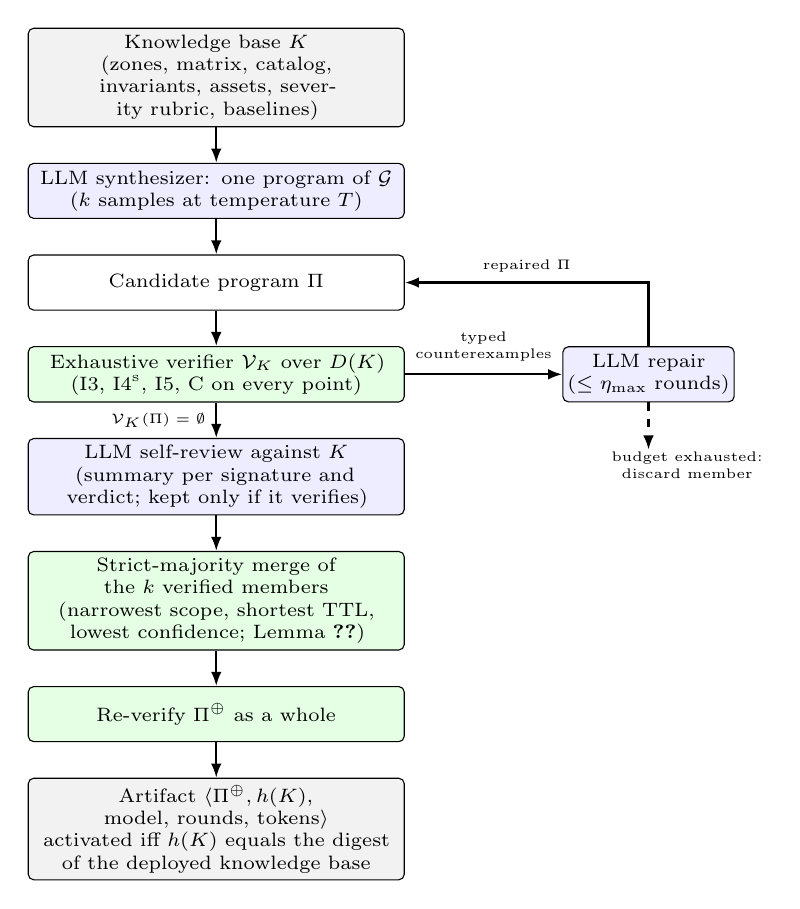
\begin{tikzpicture}[
        font=\scriptsize, node distance=4.5mm,
        st/.style={draw, rounded corners=2pt, align=center, text width=46mm, minimum height=7mm, inner sep=2.5pt, fill=white},
        llm/.style={st, fill=blue!7},
        ver/.style={st, fill=green!10},
        side/.style={draw, rounded corners=2pt, align=center, text width=20mm, minimum height=7mm, inner sep=2.5pt, fill=blue!7},
        flow/.style={-{Latex[length=1.8mm]}, thick},
        lab/.style={font=\tiny, align=center}
    ]
    \node[st, fill=gray!10] (kb) {Knowledge base $K$ (zones, matrix, catalog,\\invariants, assets, severity rubric, baselines)};
    \node[llm, below=of kb] (syn) {LLM synthesizer: one program of $\mathcal{G}$\\($k$ samples at temperature $T$)};
    \node[st, below=of syn] (cand) {Candidate program $\Pi$};
    \node[ver, below=of cand] (ver) {Exhaustive verifier $\mathcal{V}_K$ over $D(K)$\\(I3, I4$^{\mathrm{s}}$, I5, C on every point)};
    \node[llm, below=of ver] (rev) {LLM self-review against $K$\\(summary per signature and verdict; kept only if it verifies)};
    \node[ver, below=of rev] (maj) {Strict-majority merge of the $k$ verified members\\(narrowest scope, shortest TTL, lowest confidence; Lemma~\ref{lem:ensemble})};
    \node[ver, below=of maj] (rever) {Re-verify $\Pi^{\oplus}$ as a whole};
    \node[st, fill=gray!10, below=of rever] (art) {Artifact $\langle \Pi^{\oplus}, h(K),$ model, rounds, tokens$\rangle$\\activated iff $h(K)$ equals the digest of the deployed knowledge base};
    \node[side, right=20mm of ver] (rep) {LLM repair\\($\le \eta_{\max}$ rounds)};
    \draw[flow] (kb) -- (syn);
    \draw[flow] (syn) -- (cand);
    \draw[flow] (cand) -- (ver);
    \draw[flow] (ver) -- node[lab, left]{$\mathcal{V}_K(\Pi)=\emptyset$} (rev);
    \draw[flow] (rev) -- (maj);
    \draw[flow] (maj) -- (rever);
    \draw[flow] (rever) -- (art);
    \draw[flow] (ver.east) -- node[lab, above=1pt, pos=0.5]{typed\\counterexamples} (rep.west);
    \draw[flow] (rep.north) |- node[lab, pos=0.75, above]{repaired $\Pi$} (cand.east);
    \draw[flow, dashed] (rep.south) -- ++(0,-0.6) node[right, lab, anchor=west, xshift=-6mm, yshift=-2mm]{budget exhausted:\\discard member};
    \end{tikzpicture}}
    \caption{Verification-guided response synthesis (Algorithm~\ref{alg:synthesis}). Shaded blue boxes are model calls; shaded green boxes are deterministic checks. A candidate program is verified exhaustively over the finite alert domain; typed counterexamples guide repair for at most $\eta_{\max}$ rounds; verified members are merged by strict majority, re-verified as a whole, and bound to the digest of the knowledge base they were synthesized from.}
    \label{fig:loop}
\end{figure}

\begin{algorithm}[!htbp]
\caption{Verification-guided response synthesis}
\label{alg:synthesis}
\small
\begin{algorithmic}[1]
\Require knowledge base $K$; language $\mathcal{G}$; verifier $\mathcal{V}_K$; ensemble size $k$; repair budget $\eta_{\max}$; sampling temperature $T$
\Ensure verified ensemble $\Pi^{\oplus}$ bound to $h(K)$, or $\bot$
\State $M \gets \emptyset$
\For{$j = 1$ \textbf{to} $k$}
    \State $\Pi \gets \textsc{Synthesize}(K,\mathcal{G};T)$; $\eta \gets 0$ \Comment{one model call}
    \State $C \gets \mathcal{V}_K(\Pi)$ \Comment{exhaustive over $D(K)$}
    \While{$C\neq\emptyset$ \textbf{and} $\eta<\eta_{\max}$}
        \State $\Pi \gets \textsc{Repair}(\Pi, \textsc{Typed}(C))$; $\eta \gets \eta+1$ \Comment{rule, check, example input}
        \State $C \gets \mathcal{V}_K(\Pi)$
    \EndWhile
    \State \textbf{if} $C\neq\emptyset$ \textbf{then} discard $\Pi$ \textbf{and continue} \Comment{budget exhausted}
    \State $\Pi' \gets \textsc{Review}(\Pi, \textsc{Summarize}(\Pi), K)$ \Comment{self-review against $K$}
    \State \textbf{if} $\mathcal{V}_K(\Pi')=\emptyset$ \textbf{then} $\Pi \gets \Pi'$
    \State $M \gets M\cup\{\Pi\}$
\EndFor
\State \textbf{if} $M=\emptyset$ \textbf{then return} $\bot$ \Comment{all alerts take the runtime path}
\State $\Pi^{\oplus} \gets \textsc{Majority}(M)$ \Comment{Lemma~\ref{lem:ensemble}}
\State \textbf{assert} $\mathcal{V}_K(\Pi^{\oplus})=\emptyset$
\State record $h(K)$, model, repair rounds, token cost
\State \Return $\Pi^{\oplus}$
\end{algorithmic}
\end{algorithm}

\paragraph{Program language}
A program is an ordered list of rules over the eight features of Definition~\ref{def:features}: the signature (cataloged or unknown, from the alert), the severity (P1 to P4, from the alert), the source and destination zones (from the topology) with the derived policy verdict (allow, deny, intra-zone, or external, from the matrix), the protected-source flag (from the invariants), and the three history counts (prior alerts of the source, other targets of the source, and other ports on the target, from the alert history), with first-match semantics and the outcomes of Section~\ref{sec:synthesis_problem}. The scope of a \textsc{drop} selects only the destination and port (flow, pair, or host); the language has no target field, so an enforced rule always blocks the alert source as a single host. Each \textsc{drop} rule carries a rationale and the knowledge-base entries it relies on, which form its audit trace at runtime.

\paragraph{Exhaustive verification}
For the deployed fabric, 29 signatures and the unknown value, four severities, nine zones including external, the protected flag, and seven consistent history combinations give $|D(K)|=136{,}080$ points, of which $|R(K)|=19{,}824$ can be emitted by the deployed IDS. The verifier evaluates the program on every point and returns every violation of I3, I4$^{\mathrm{s}}$, I5, or C (Definition~\ref{def:verifier}) as a typed counterexample naming the rule, the check, and an example input. Verifying one program takes about five seconds on the testbed host.

\paragraph{Synthesis and repair}
The synthesizer gives the LLM the knowledge-base documents and the language definition and asks for one program that covers the whole fabric. The objectives are stated in priority order: obey the hard constraints, contain what the knowledge base identifies as requiring response, do not cut traffic it documents as legitimate, prefer the narrowest scope, and abstain when the knowledge base does not determine the answer. A rejected program is returned to the model with its typed counterexamples, and the model repairs it for at most $\eta_{\max}$ rounds; a program that still fails is discarded, which reduces the ensemble to the members that verified, and if no member verifies the synthesis returns no program and all alerts take the runtime path until the next attempt. This is the counterexample-guided loop of CEGIS~\cite{solarlezama2006sketching} with an LLM as the inductive synthesizer and an exhaustive rather than symbolic verifier.

\paragraph{Self-review}
A verified program is summarized per signature and policy verdict, and the model reviews this behavior against the knowledge base. The review targets the second synthesis objective, agreement with the documented response, which the verifier does not check; the revision is kept only if it also verifies.

\paragraph{Ensemble}
Because sampled programs differ, BIZM synthesizes $k$ programs independently and deploys their point-wise strict majority as defined in Lemma~\ref{lem:ensemble}: an action is taken only when a strict majority chooses it, otherwise the ensemble abstains, and among agreeing programs the narrowest scope, shortest TTL, and lowest confidence are kept. The ensemble is verified again as a whole.

\paragraph{Activation and runtime use}
The synthesized artifact records the digest of the knowledge base it was synthesized from, the model, the repair rounds, and the token cost. The agent activates a program only if it was verified at synthesis time, its digest equals that of the running knowledge base, and it passes verification again in the agent process. A knowledge-base change therefore disables the old program until it is resynthesized, and all alerts take the runtime path in the meantime. At runtime, the features are extracted from the alert and from the source's alerts in the preceding ten minutes. A program decision becomes a bounded intent whose audit trace is the rule rationale and its cited entries, and it passes the validators, rate limits, circuit breaker, and enforcement path of Section~\ref{sec:decision_safety}. Any error on the compiled path falls back to the runtime path rather than failing the alert.

\subsection{Runtime Reasoning and Safety Validation}
\label{sec:decision_safety}

Alerts on which the program abstains, and all alerts while no verified program is active, take the runtime path. It is a structured pipeline of six functions: alert classification, context retrieval, LLM reasoning, safety validation, enforcement planning, and rule generation; the last three are shared with the compiled path. Contextual interpretation benefits from an LLM, whereas schema checking, target binding, TTL enforcement, protected-asset exclusion, blast-radius checking, and rule construction must remain deterministic.

\paragraph{Alert classification}
Processing begins with normalization and deduplication. The Suricata EVE JSON alert is mapped to the response schema (source and destination addresses, protocol, destination port, signature, category, severity, timestamp), and duplicates within a suppression window are ignored. Alerts reach the classifier only when the program abstains. The classifier assigns a coarse response class: low-severity or duplicate events follow a log-only path, while high-priority alerts proceed to context retrieval and reasoning. This filter reduces unnecessary LLM calls and avoids enforcement attempts for events that are not eligible for automated containment.

\paragraph{Graph-grounded context}
The context engine supplies the reasoning component with a constrained factual context rather than raw network state. The context graph includes zones, assets, leaf-switch attachment, IDS signatures, active DROP rules, protected address ranges, baseline communication edges, and prior incidents. For each alert it retrieves the source and destination zones, the policy-matrix entry, active rules, protected-asset status, recent similar incidents, and the expected impact of blocking the source. This gives the LLM the factual substrate needed to distinguish legitimate permitted-path behavior from suspicious behavior on the same allowed edge, and limits prompt exposure by supplying only the context needed for the current decision. The graph-query interface is read-only; any state-changing operation is outside the agent's tool set.

\paragraph{LLM reasoning}
The reasoning engine evaluates the alert in context and produces a candidate bounded-isolation decision. The model is signature-informed but not signature-keyed: for known signatures the prompt includes trusted metadata such as severity, category, MITRE mapping, and expected disposition, but reasoning is reserved for the cases where static mapping is brittle, including permitted-path anomalies, unknown signatures, conflicting evidence, and scope selection under safety constraints. The output is schema-split: the enforcement-facing output is a compact structured action containing only the fields needed for validation and rule generation: the action (DROP or NONE), the source address, which must equal the alert source, the destination address, protocol, and destination port, a TTL in $[60,3600]$ seconds, a confidence in $[0,1]$, and the ATT\&CK tactic and technique for audit, while the audit-facing output records the rationale, supporting evidence, alternatives, and follow-up recommendations. This split reduces parser failures and prevents a long explanation from delaying the enforcement path.

The runtime path keeps a decision cache for repeated alerts. An enforced decision is cached for 60 seconds under a key of signature, source, destination, port, protocol, and correlation signal. On a hit, the cached intent is rebound to the source of the current alert and passes validation again; alerts for a flow already covered by an active agent rule are suppressed until the rule expires. The cache saves a model call only within this window, whereas the compiled path removes it for every covered alert.

\paragraph{Fail-closed validation}
The validator applies the invariants of Section~\ref{sec:invariants}. It checks schema conformance, sanitizes alert-derived text, verifies that the source exists in the context graph, rejects duplicate or conflicting rules, enforces the protected-asset set, rejects off-target isolation, clamps TTL to the configured interval, applies severity and confidence gates, and enforces per-source and global blast-radius limits. Any failed check results in non-enforcement and audit recording.

Prompt-injection handling has three layers. First, only the signature and category text are attacker-influenced; the prompt places them in a delimited untrusted-data block, while addresses, zones, port, signature identifier, and severity come from the parsed packet header and are marked as trusted. Second, the two text fields are scored against 15 patterns, including instruction overrides, role and chat-template tags, target coercion such as ``block'' followed by an address, and hidden Unicode characters; a field that matches two or more is redacted before it reaches the model. Third, and decisively, the enforcement target is bound to the header source after the model returns and checked against $\mathcal{N}$, so an instruction that passes the filter can change at most whether the source is contained, never which host is blocked. The compiled path does not read the alert text at all.

\paragraph{Enforcement planning and rule generation}
Only an admissible decision is converted into a DROP intent. The enforcement planner binds the decision to the alert source, protocol, destination port, TTL, provenance metadata, and source-side enforcement scope, and the rule generator converts the intent into a policy/YANG-oriented request for the control plane. The model proposes the bounded action; deterministic components decide whether it is admissible and how it is represented for enforcement. Algorithm~\ref{alg:decision} summarizes the complete decision logic.

\begin{algorithm}[!t]
\caption{Fail-closed bounded-isolation decision}
\label{alg:decision}
\small
\begin{algorithmic}[1]
\Require alert $a=(s,d,\rho,\pi,\sigma,\ell,\kappa,\tau,t)$; policy $P$; baseline $B$; protected set $\mathcal{N}$; active rules $\mathcal{R}$; program $\Pi^{\oplus}$ (if active); threshold $\tau_c$; TTL bounds $[\delta_{\min},\delta_{\max}]$; blast-radius limits $\mathcal{L}$
\Ensure an authorized, provenance-marked bounded \textsc{drop} rule, or a non-enforcing decision \textsc{none}/\textsc{log\_only}
\State $a' \gets \textsc{NormalizeAndDeduplicate}(a)$
\If{$a'$ is invalid or duplicated within the suppression window}
    \State $o \gets \textsc{none}$
\ElsIf{$\ell \notin \{\text{P1},\text{P2}\}$}
    \State $o \gets \textsc{log\_only}$
\Else
    \State $u \gets \Pi^{\oplus}(\phi_K(a',\textsc{History}(s)))$ \Comment{compiled path}
    \If{$\Pi^{\oplus}$ is inactive or $u.\alpha = \textsc{abstain}$} \Comment{runtime path}
        \State $ctx \gets \textsc{RetrieveContext}(a',P,B,\mathcal{R})$
        \State $ctx \gets ctx \cup \textsc{Neighbors}(s) \cup \textsc{SimilarIncidents}(a') \cup \textsc{BlockImpact}(s)$
        \If{\textsc{CacheHit}$(a')$}
            \State $u \gets \textsc{CachedDecision}(a')$
        \Else
            \State $u \gets \textsc{LLMDecision}(a',ctx)$
        \EndIf
    \EndIf
    \If{$u$ fails schema validation}
        \State $o \gets \textsc{none}$
    \ElsIf{$u.\alpha \neq \textsc{drop}$}
        \State $o \gets \textsc{log\_only}$
    \ElsIf{$u.\theta \neq s$ or $u.\theta \in \mathcal{N}$}
        \State $o \gets \textsc{none}$
    \ElsIf{\textsc{ConflictOrDuplicate}$(u,\mathcal{R})$}
        \State $o \gets \textsc{none}$
    \ElsIf{$u.c < \tau_c$}
        \State $o \gets \textsc{log\_only}$
    \ElsIf{\textsc{BlastRadiusExceeded}$(u,\mathcal{L})$ or \textsc{CircuitBreakerOpen}()}
        \State $o \gets \textsc{none}$
    \Else
        \State $u.\delta \gets \textsc{Clamp}(u.\delta,\delta_{\min},\delta_{\max})$
        \State $r \gets \textsc{GenerateDropIntent}(u,\textsc{agent})$
        \State $o \gets \textsc{AuthorizeAndEnforce}(r)$
    \EndIf
\EndIf
\State \textsc{RecordAudit}$(a',u,o)$
\end{algorithmic}
\end{algorithm}

\subsection{Zero Trust Enforcement Plane}
\label{sec:enforcement_plane}

The enforcement plane prevents the LLM Security Agent from becoming an over-privileged network operator. The control path consists of the IDS Agent, the Secure Framework, and ONAP SDN-C. The IDS Agent integrates the decision layer with the control plane; the Secure Framework mediates policy requests using mTLS and RBAC; ONAP SDN-C acts as the policy controller that coordinates accepted operations and fabric-side enforcement.

Figure~\ref{fig:secure_framework} details the enforcement boundary. The LLM Security Agent does not send device commands. An accepted DROP intent is submitted to the IDS Agent and forwarded to the Secure Framework through a restricted REST interface. The Secure Framework authenticates the request, binds it to a restricted service identity, checks command-level authorization, validates the operation against the YANG model, attaches provenance metadata, and translates the accepted intent into a gNMI-compatible operation, which is pushed to the data-plane switch through a mutually authenticated gRPC/gNMI channel.

\begin{figure}[t]
    \centering
    \includegraphics[width=\columnwidth]{figs/framework.pdf}
    \caption{Identity-aware Secure Framework of the BIZM enforcement plane. The framework receives authorized bounded-response requests through a restricted northbound interface, validates operations against the YANG model, checks service-account permissions at command granularity under the restricted response role, translates accepted operations into gNMI/protobuf requests with provenance metadata, and pushes device-level rules to the data-plane switch through a mutually authenticated gRPC/gNMI channel. ACCEPT rules, deletions, unsupported operations, and requests without a valid identity fail closed at the authorization step.}
    \label{fig:secure_framework}
\end{figure}

The control-plane contract is intentionally narrow. BIZM can create temporary DROP rules, but it cannot create ACCEPT rules, delete unrelated rules, modify baseline segmentation policy, change routing state, or access protected management objects. Each accepted rule must be source-faithful, DROP-only, time-bounded, provenance-marked, and authorized under the restricted response role. Requests that target protected assets, request unsupported operations, lack valid credentials, or violate the allowed command set fail closed before reaching the fabric.

\subsection{End-to-End Workflow}
\label{sec:e2e_workflow}

The end-to-end workflow follows the six steps of Section~\ref{sec:arch_overview}. It is closed-loop but not unrestricted: each iteration is bounded by action type, target fidelity, TTL, protected-asset exclusion, confidence threshold, severity threshold, blast-radius limit, identity-aware authorization, and audit recording. The response is reversible because each rule has an explicit lifetime; when the TTL expires, the agent revokes the temporary rule, and the baseline segmentation policy remains unchanged.

Consider a compromised APP-CORE host that abuses its permitted database path to DB-OLTP. The static policy allows the zone pair, so the fabric does not block the flow by default. If Suricata raises a cataloged content signature, such as destructive SQL, the synthesized program issues a flow-scope DROP on the source without a model call. If the alert instead carries an unknown signature for a high-rate bulk transfer, the program abstains, and the runtime path retrieves the APP-CORE to DB-OLTP baseline, recent similar incidents, active rules, source leaf attachment, protected-asset status, and block-impact context. Because the edge is permitted, the response is not a fixed lookup: the reasoning engine compares the observed behavior with the baseline and proposes a bounded DROP on the source. In both cases, the validator confirms that the target equals the alert source, the source is not protected, the TTL is within bounds, and the confidence and severity gates are satisfied, and the rule generator emits a DROP intent that is authorized by the Secure Framework, coordinated through ONAP SDN-C, and enforced at the source-side leaf. A legitimate DB-OLTP replication burst toward DB-ANALYTICS, by contrast, matches the baseline and is recorded without enforcement.

This workflow captures the main design principle of BIZM: use the LLM to synthesize what the knowledge base determines and to reason where it does not, but constrain every consequential action through deterministic validation and Zero Trust enforcement.

\section{Implementation and Experimental Design}
\label{sec:implementation_experiment}

\subsection{Testbed Implementation}
\label{sec:testbed_implementation}

We implement BIZM on a virtualized spine-leaf data-center fabric emulated in GNS3 with SONiC switches~\cite{sonic2026}. Static microsegmentation is enforced as deny-by-default rules on the leaf switches, and runtime containment is installed as a temporary source-side DROP rule at the leaf nearest the suspicious workload. Each automated rule carries a TTL and provenance metadata, and the agent revokes it when the TTL expires.

Suricata monitors mirrored east-west traffic and exports EVE JSON alerts~\cite{oisf2026suricata}. The IDS is placed off the forwarding path: it supplies the suspicious signal, while BIZM performs response-level decision making, following the common pattern in which lightweight sensing provides the initial evidence and deeper analysis runs outside the packet-forwarding path~\cite{cSDAID22,jSAID23,jAPELID24}. An IDS Agent subscribes to the alert stream, forwards normalized alerts to the decision plane, receives admissible DROP intents, and records live status for the operator dashboard.

Enforcement success is verified through four checks: the rule appears in the device rule datastore, the intended source can no longer reach the target service, unrelated traffic remains unaffected, and the installed rule carries the expected TTL and provenance mark. This distinguishes correct containment from accidental reachability loss or over-broad blocking. The verifier, synthesizer, and ensemble code of Algorithm~\ref{alg:synthesis} run on the control-plane host, a virtual machine with 32 vCPUs of an Intel Xeon (Cascade Lake) processor and 94 GB of memory.

\subsection{BIZM Configuration}
\label{sec:runtime_configuration}

The runtime policy follows the eight-zone matrix of Table~\ref{tab:policy_matrix}. The protected set $\mathcal{N}$ includes management hosts, monitoring hosts, IDS components, zone gateways, and control-plane components. Automatic enforcement is allowed only for P1 and P2 alerts. The runtime confidence threshold is $\tau_c=0.70$: a decision at or above 0.85 is enforced, one between 0.70 and 0.85 is enforced with an operator notification, one between 0.50 and 0.70 is held for review, and a lower one is rejected. The compiled path requires $\tau_\Pi=0.85$, and 0.90 for a \textsc{drop} that overrides a permitted path. Algorithm~\ref{alg:decision} shows the single gate $\tau_c$; the notification and hold bands are implemented inside \textsc{AuthorizeAndEnforce} and \textsc{RecordAudit} and do not change which decisions reach the fabric. Each DROP rule has a TTL in $[60,3600]$ seconds. Blast-radius limits are five automated rules per minute, fifty active automated rules in total, and three rules per source address within five minutes. A circuit breaker pauses enforcement after three consecutive failed enforcement attempts.

The LLM is \texttt{gpt-oss-120b}, an open-weight mixture-of-experts model with about 117 billion parameters. The synthesizer uses it with \texttt{reasoning\_effort} set to medium. Its input is the knowledge base of seven documents (zones, policy matrix, signature catalog, invariants, assets, severity rubric, and baselines), about 22K tokens. The deployed program is a strict-majority ensemble of $k=5$ programs sampled at temperature 0.7, each repaired for at most $\eta_{\max}=3$ rounds and reviewed once. Synthesis at temperature 0 is also reported as a single-program configuration. \red{For the cross-model experiment (Section~\ref{sec:cross_model}), the same synthesis configuration is run with [Qwen model id].}

On the runtime path, the same model serves both the reasoning and the classification roles, with \texttt{reasoning\_effort} set to low. The reasoning call uses temperature 0.1, at most 3072 output tokens, and a 15-second timeout, and each P1/P2 alert receives a single reasoning call without self-consistency voting. The classification call uses temperature 0.0 and at most 1024 output tokens, and handles early severity/category filtering; duplicate alerts with the same source and signature are suppressed for 30 seconds. The reasoning prompt has four parts: trusted alert metadata, the untrusted alert text in its delimited block, the retrieved context with recent alerts from the same source, and the output schema. Prompts are fixed across runs, and no scenario-specific prompt tuning is performed. The enforcement-facing output is constrained by the structured decision schema of Section~\ref{sec:decision_safety}; the reasoning trace is recorded for audit but is not used to authorize enforcement.

\subsection{Research Questions, Scenarios, and Baselines}
\label{sec:scenarios_baselines}

The evaluation addresses six questions.
\begin{itemize}[leftmargin=*]
    \item \textbf{RQ1 (Synthesis fidelity).} Does verification-guided synthesis produce a verified program that agrees with the knowledge base, and what does the verifier catch that the synthesizer alone would have deployed?
    \item \textbf{RQ2 (Robustness to change).} Does resynthesis keep the program correct when the knowledge base changes?
    \item \textbf{RQ3 (Sensitivity).} How do ensemble size and model choice affect coverage, agreement, and synthesis cost?
    \item \textbf{RQ4 (Live containment).} Does BIZM contain functional east-west threats on the live testbed, at what latency, and at what cost to legitimate traffic?
    \item \textbf{RQ5 (Adversarial safety).} Does the safety mechanism prevent unsafe enforcement under alert manipulation and under a coordinated multi-source campaign?
    \item \textbf{RQ6 (Residual reasoning and scalability).} How does the runtime path handle alerts the program does not cover, what does each path cost, and how does verification scale with the fabric?
\end{itemize}

RQ1 to RQ3 are evaluated offline over the alert domain. For RQ2, four modified copies of the knowledge base represent changes an operations team makes between syntheses: six new signatures, two of which detect abuse inside permitted connections (V1); a ninth crown-jewel zone, PAYMENTS, with its matrix rows, gateway, and two zone-pair signatures (V2); three documented responses changed in prose only (V3); and all three changes together (V4). Each variant is resynthesized, while the baselines are left as written. For RQ3, the ensemble size is varied over $k\in\{1,3,5,7,9\}$ with 20 ensembles per $k$ drawn without replacement from the pool of 30 syntheses, \red{and the synthesis configuration is repeated with a second open-weight model.}

Table~\ref{tab:scenarios} summarizes the testbed scenarios. Five scenarios use live east-west traffic and exercise the full detection-to-enforcement path. Five scenarios use controlled injected alerts to stress the decision logic, protected-asset handling, prompt-injection resistance, policy-matrix coverage, unknown signatures, and multi-stage correlation. Live scenarios are repeated ten times. Injected scenarios are repeated three times with the synthesized program, whose decisions are deterministic, and ten times in the runtime-only configuration. These repetitions measure run-to-run stability and should not be interpreted as a large independent traffic corpus. A matrix sweep injects 75 alerts generated mechanically from every off-diagonal cell of the policy matrix, the signature catalog, and the protected set, five times each. \red{Scenario S11 launches a coordinated campaign from $n_s\in\{3,5,8,12\}$ non-protected sources within 60 seconds and is repeated [$N$] times per $n_s$.}

\begin{table}[t]
    \centering
    \caption{Evaluation scenarios and repetitions ($N$: BIZM/runtime-only).}
    \label{tab:scenarios}
    \footnotesize
    \setlength{\tabcolsep}{3pt}
    \begin{tabularx}{\columnwidth}{@{}l>{\raggedright\arraybackslash}X>{\raggedright\arraybackslash}p{2.0cm}c@{}}
        \toprule
        \textbf{ID} & \textbf{Description} & \textbf{Type} & \textbf{N} \\
        \midrule
        S1  & WEB to DB-OLTP direct, application-chain bypass & Denied-cell violation & 10/10 \\
        S2  & APP-CORE reverse connection to WEB & Denied-cell lateral movement & 10/10 \\
        S3  & DB-OLTP outbound beacon from sink tier & Denied-cell behavioral violation & 10/10 \\
        S4  & Destructive SQL on permitted APP-CORE to DB-OLTP edge & Permitted-path anomaly & 10/10 \\
        S5  & Management and monitoring baseline traffic & Legitimate FP control & 10/10 \\
        S6  & Denied-cell injections and legitimate flows & Matrix coverage and FP & 3/10 \\
        S7  & Prompt injection, severity bypass, spoofed-source alerts & Adversarial safety & 3/10 \\
        S8  & Protected management or monitoring host acting maliciously & Never-block invariant & 3/10 \\
        S9  & Known, unknown, and legitimate signatures & Reasoning ablation & 3/10 \\
        S10 & Three-stage campaign from a single source & Kill-chain correlation & 3/10 \\
        \red{S11} & \red{Coordinated campaign from $n_s$ sources within 60 s (direct and spoofed-decoy variants)} & \red{Blast-radius exhaustion} & \red{[N]/[N]} \\
        \bottomrule
    \end{tabularx}
\end{table}

We compare BIZM against three baselines and one ablation.
\begin{itemize}[leftmargin=*]
    \item \emph{SOAR-A} is a signature-keyed responder that issues a DROP against the alert source for a fixed set of known-dangerous signatures and takes no action otherwise; a host-isolation variant is used in the matrix sweep. It represents fixed playbooks.
    \item \emph{Baseline-B} uses the same LLM decision model as BIZM but removes deterministic safety validation and least-privilege enforcement. It receives raw alert text and emits an action directly, which isolates the contribution of the safety controls.
    \item \emph{Baseline-C} is a deterministic contextual rule written by the authors over the same topology, policy matrix, and protected set: it contains a severe alert on a denied zone pair and, on a permitted pair, only for a hand-written list of abuse signatures. It is evaluated as deployed, with zone-level protection of MGT and MONITORING, and in a strongest variant that protects exactly the hosts of the protected set and reads zones and the matrix from the current knowledge base. It separates the contribution of the LLM from that of the context itself.
    \item \emph{Runtime-only} is BIZM with the synthesized program disabled, so every alert is reasoned by the LLM. This ablation isolates the compiled path.
\end{itemize}

\subsection{Evaluation Metrics}
\label{sec:evaluation_metrics}

For response correctness, each labeled decision is classified as TP, FP, TN, or FN. A positive case is a true threat whose correct response is a bounded DROP decision~\cite{jSAID23}; a negative case is benign, ambiguous, low-severity, or unsafe to enforce and should not trigger automated containment. We report precision, threat-containment rate (TCR), F1-score, false positive rate (FPR), and accuracy:
\[
\mathrm{Precision}=\frac{\mathrm{TP}}{\mathrm{TP}+\mathrm{FP}},
\quad
\mathrm{TCR}=\frac{\mathrm{TP}}{\mathrm{TP}+\mathrm{FN}},
\]
\[
\mathrm{F1}=\frac{2\cdot \mathrm{Precision}\cdot \mathrm{TCR}}
{\mathrm{Precision}+\mathrm{TCR}},
\quad
\mathrm{FPR}=\frac{\mathrm{FP}}{\mathrm{FP}+\mathrm{TN}}.
\]
TCR is a response-level metric: it measures the fraction of true threat cases for which the system issues an admissible bounded DROP decision, and it should not be interpreted as an IDS detection rate, because BIZM operates after an alert has been generated.

For RQ1 to RQ3, ground truth is derived mechanically from the knowledge base, never from a program. For an alert with a cataloged signature, the documented response governs: a documented \textsc{drop} means contain, a documented log-only means do not contain, and a \textsc{drop} conditioned on correlation means contain only after a prior alert from the source. Protected or external sources and P3 or P4 alerts are never contained. Points the knowledge base does not settle are left ungraded: a correlation-conditioned signature with no prior alert, and a log-only signature of severity P1 or P2 on a denied pair, where the pair itself is a policy violation. Unknown signatures are reported separately. On the graded points we report \emph{accuracy} over the points a system decides and \emph{coverage}, the fraction it decides rather than abstains on. Because these results enumerate the domain rather than sample it, they carry no sampling interval. For the synthesis loop we additionally report the verification outcome of each candidate program, the number and invariant type of counterexamples per round, the repair rounds used, whether the self-review revision was accepted, and the agreement and coverage of the \emph{unverified} candidates, that is, of what the synthesizer would have deployed without the verifier.

We also report the following metrics.
\begin{itemize}[leftmargin=*]
    \item \textbf{Latency.} Detection latency from traffic onset to the IDS alert; decision latency from alert ingestion to a decision accepted by the Secure Framework; enforcement latency from that decision to rule visibility in the leaf datastore. Medians, 95th percentiles, and empirical distributions are reported.
    \item \textbf{Exposure.} For the matrix sweep, the service edges a rule closes and the legitimate baseline flows it cuts.
    \item \textbf{Safety.} Safety-violation rate, protected-service availability, never-block respect for protected assets, and, for the multi-source campaign, the fraction of sources contained before and after blast-radius saturation.
    \item \textbf{Reasoning.} Correct-decision rates on known and unknown signatures.
    \item \textbf{Overhead.} Median and tail decision latency, model tokens per decision, the one-time cost of synthesis, verifier time as a function of $|D(K)|$, and sustained compiled-path throughput.
\end{itemize}
Proportions are reported with exact Clopper-Pearson 95\% intervals, and paired comparisons with the exact McNemar test.

\section{Results, Evaluation, and Discussion}
\label{sec:results_discussion}

\subsection{Synthesis Fidelity: Agreement with the Knowledge Base (RQ1)}
\label{sec:compiled_fidelity}

Table~\ref{tab:agreement} compares synthesized programs with Baseline-C over the deployed knowledge base (V0) and, for RQ2, over its four variants. Of the 19,824 realizable points of V0, 14,970 are graded, 822 are ungraded, and 4,032 carry an unknown signature. Every deployed program passed verification with no violating point. The single program synthesized at temperature 0 decides 97.5\% of the graded points and agrees with the knowledge base on all of them, and it was identical across five syntheses. The ensemble decides every graded point and agrees on all of them. Its members varied individually, with coverage between 69.0\% and 100\% and one member missing 966 contain points, and the strict-majority vote removed every member error, as Lemma~\ref{lem:ensemble} guarantees for safety and as the data show for agreement.

\begin{table}[t]
    \centering
    \caption{Agreement with the knowledge base on the deployed snapshot V0 and after the four changes V1 to V4 (BIZM resynthesized, Baseline-C unchanged). Graded: graded points of the snapshot.}
    \label{tab:agreement}
    \scriptsize
    \setlength{\tabcolsep}{1.8pt}
    \begin{tabular}{@{}lccccc@{}}
        \toprule
        & & \multicolumn{2}{c}{\textbf{Baseline-C}} & \multicolumn{2}{c}{\textbf{BIZM}} \\
        \cmidrule(lr){3-4}\cmidrule(l){5-6}
        \textbf{Knowledge base} & \textbf{Graded} & \textbf{Depl.} & \textbf{Strong.} & \textbf{Acc.} & \textbf{Cov.} \\
        \midrule
        V0, single ($T{=}0$) & 14,970 & 94.54\% & 96.07\% & 100.00\% & 97.5\%  \\
        V0, ensemble ($k{=}5$) & 14,970 & 94.54\% & 96.07\% & 100.00\% & 100.0\% \\
        V1 new signatures            & 19,520 & 93.73\% & 94.98\% & 100.00\% & 95.0\%  \\
        V2 new zone                  & 18,705 & 93.03\% & 96.26\% & 100.00\% & 97.5\%  \\
        V3 prose retuning            & 15,034 & 94.46\% & 96.09\% & 100.00\% & 100.0\% \\
        V4 all changes               & 24,428 & 92.03\% & 95.24\% & 99.97\%  & 92.3\%  \\
        \bottomrule
    \end{tabular}
\end{table}

Baseline-C errs in both directions. Its hand-written list of permitted-path abuse signatures includes three signatures that the catalog documents as log-only, so even its strongest variant blocks 588 points that the knowledge base says to log (no false negatives, 588 false positives). The deployed variant also protects every host of MGT and MONITORING instead of the hosts in the protected set and misses 544 contain points (544 false negatives, 273 false positives), and it enforces on 518 points with an unknown signature, which BIZM defers to the runtime path. The rule is consistent with the policy matrix but not with the prose of the catalog, which it never reads. The synthesized program is derived from that prose, and this is where the LLM contributes. Synthesizing the ensemble took 117 seconds and 341K tokens. A mechanically compiled program that reads only the structured fields of the catalog, without the LLM, agrees with the knowledge base on 93.55\% of the graded points when it must decide all of them, missing 966 contain points on permitted and outbound pairs, or agrees on all of the 89.6\% it can decide when it abstains elsewhere; on V1 to V4 the same program reaches 93.0\% to 93.9\%, or 100\% at 88.6\% to 90.2\% coverage. This bounds the contribution of the LLM to the roughly 10\% of graded points whose response is stated only in the prose of the catalog.

\paragraph{What the verifier catches}
The upper part of Table~\ref{tab:loop} reports the dynamics of Algorithm~\ref{alg:synthesis} for the six syntheses of the deployed knowledge base (five ensemble members and the temperature-0 program). Of the six initially synthesized programs, three failed verification at round 0 with 24 counterexamples in total (15, 3, and 6), covering 18,648 violating inputs; one repair round sufficed for each of them, and no candidate was discarded. The self-review revision verified and was kept for all six programs; it raised the coverage of the realizable points for three ensemble members, from 91.0\% to 92.1\%, from 88.7\% to 95.5\%, and from 85.9\% to 90.9\%. The round-0 candidates of these syntheses were not retained, so the following figures come from a pool of 30 further syntheses of V0 at $T=0.7$ in which every candidate was kept. Eight of the 30 failed verification at round 0 with 47 counterexamples, 41 of them on the TTL and scope check I4$^{\mathrm{s}}$, four on I5, and two on I3; every one was repaired within two rounds (0.33 on average), and none was discarded. The eight unverified round-0 candidates agreed with the knowledge base on 98.75\% of the graded points they decided, against 100\% for the 22 that verified at once, and one of them would have issued 448 unsafe \textsc{drop} decisions on protected sources, which quantifies what verification-guided repair removes before deployment. Self-review changed the decision on 257 to 3,736 graded points (median 680) in 15 of the 30 syntheses.

\paragraph{Synthesis ablation}
The lower part of Table~\ref{tab:loop} isolates the contribution of each stage of the loop over the pool of 30 independent syntheses of V0 at temperature 0.7, read at four stages: one-shot synthesis with no verifier feedback, repair only, repair with self-review, and the full ensemble of five. One-shot candidates verify in only 73.3\% of the cases, agree with the knowledge base on 99.67\% of the graded points they decide (95\% CI over syntheses [99.17, 100]), and include 448 unsafe \textsc{drop} decisions; repair raises the verification rate to 100\% (exact McNemar $p=0.008$ on the eight discordant syntheses) and removes every unsafe decision while leaving agreement on decided points essentially unchanged at 99.77\%; self-review raises agreement to 100.00\% and coverage from 93.6\% to 96.7\%; and ensembles of five raise coverage to 99.6\% (95\% CI [99.0, 100]) at 100\% agreement. The same ablation on a pool of 20 syntheses of V4 gives 70\% verified at round 0 (one draft could not be parsed), no unsafe decision at any stage, agreement of 99.80\%, 99.64\%, and 99.68\% for the three single-program stages, and 100.00\% agreement at 98.9\% coverage for ensembles of five. This is the direct evidence for the title claim: the verifier, not the synthesizer, is what makes the deployed program safe, and the ensemble, not any single sample, is what makes it nearly complete.

\begin{table}[t]
    \centering
    \caption{Synthesis-loop dynamics for the six deployed syntheses (upper part) and synthesis ablation over 30 syntheses at $T=0.7$ (lower part).}
    \label{tab:loop}
    \scriptsize
    \setlength{\tabcolsep}{1.4pt}
    \begin{tabular}{@{}lcccccc@{}}
        \toprule
        \textbf{Candidate} & \textbf{CE$_0$/Ver.} & \textbf{Rnds} & \textbf{Acc.} & \textbf{Cov.} & \textbf{Unsafe} & \textbf{Tok.} \\
        \midrule
        \multicolumn{7}{@{}l}{\emph{Deployed syntheses (round-0 candidate before repair)}} \\
        $T{=}0$ single & 15 & 1 & n/a & n/a & n/a & 96K \\
        Member 1 & 0 & 0 & n/a & n/a & 0 & 54K \\
        Member 2 & 3 & 1 & n/a & n/a & n/a & 93K \\
        Member 3 & 0 & 0 & n/a & n/a & 0 & 54K \\
        Member 4 & 6 & 1 & n/a & n/a & n/a & 80K \\
        Member 5 & 0 & 0 & n/a & n/a & 0 & 60K \\
        \midrule
        \multicolumn{7}{@{}l}{\emph{Ablation arms (output the arm would deploy; mean, 95\% CI)}} \\
        One-shot (no verifier) & 73.3\% & 0 & 99.67\% & 94.3\% & 448 & 26K \\
        Repair only              & 100\% & 0.33 & 99.77\% & 93.6\% & 0 & 36K \\
        Repair + review          & 100\% & 0.33 & 100.00\% & 96.7\% & 0 & 66K \\
        Ensemble ($k{=}5$)       & 100\% & 0.26 & 100.00\% & 99.6\% & 0 & 322K \\
        \bottomrule
        \multicolumn{7}{@{}p{0.97\columnwidth}@{}}{\footnotesize Upper part: CE$_0$ is the number of counterexamples at round 0 (breakdown by check in the text), Rnds the repair rounds used, and Acc./Cov./Unsafe the agreement, coverage, and unsafe \textsc{drop} decisions (protected or external source) of the \emph{unverified} round-0 candidate on the graded points, which were not retained for these syntheses (n/a). Lower part: Ver.\ is the fraction of arm outputs with $\mathcal{V}_K(\Pi)=\emptyset$ and Rnds the mean repair rounds; Acc./Cov./Unsafe refer to what the arm would deploy, as means over the 30 syntheses (20 ensembles of five drawn from them).}
    \end{tabular}
\end{table}

\subsection{Resynthesis under Knowledge-Base Change (RQ2)}
\label{sec:drift}

Rows V1 to V4 of Table~\ref{tab:agreement} report the four knowledge-base changes. Resynthesis keeps agreement at 100\% on V1 to V3 and at 99.97\% on V4. The seven V4 errors concern SID 9000012 on PAYMENTS to DB-OLTP: the variant permits that pair but leaves the signature's detection logic unchanged, so the knowledge base contradicts itself there. Baseline-C, which is not rewritten, misses the two new abuse signatures of V1 and keeps blocking SID 9000050 after V3 documents it as log-only. Its deployed variant cannot place the PAYMENTS zone and misses 1,009 contain points in V2. The strongest variant follows the new zone and matrix rows, which are structured, but not changes stated in prose. The ensemble coverage falls to 92.3\% on V4 because its members disagree on some new signatures, and those points go to the runtime path rather than to a wrong decision. Each resynthesis took under four minutes, whereas the rule requires a code change and redeployment. The verifier rejected 8 of the 20 initial ensemble candidates across the four variants (2, 2, 1, and 3 for V1 to V4), each of which was repaired within two rounds, and no candidate was discarded; the four temperature-0 programs verified at round 0.

\subsection{Sensitivity to Ensemble Size and Model Choice (RQ3)}
\label{sec:cross_model}

\paragraph{Ensemble size}
The upper part of Table~\ref{tab:sensitivity} varies $k$. By Lemma~\ref{lem:ensemble} every ensemble is verified; what changes is the coverage-abstention trade-off and the synthesis cost. Coverage rises from 96.1\% at $k=1$ to 99.6\% at $k=5$, peaks at 99.9\% for $k=7$, and falls to 99.5\% at $k=9$, where a strict majority is harder to reach; agreement on decided points remains 100\% for every $k$, and the one-time token cost grows linearly in $k$. At $k=5$, 88\% of the abstained points carry one of the three permitted-path signatures that the catalog documents as log-only (SIDs 9000051, 9000052, and 9000061), mostly for sources with earlier alerts, where members disagree whether correlation turns logging into containment. These are exactly the points on which the knowledge base is least explicit, and the same three signatures that Baseline-C blocks.

\paragraph{Model choice}
The lower part of Table~\ref{tab:sensitivity} repeats the synthesis with a second open-weight model, \red{[Qwen model id]}, under the same prompts, budget, and verifier. \red{Qwen reaches verification in [r$_B$] rounds on average, [n$_B$] of its candidates were discarded after $\eta_{\max}$ rounds, and its ensemble agrees with the knowledge base on [a$_B$]\% of the points it decides, with coverage [c$_B$]\%. Across both models, the verifier never admitted a program with an unsafe decision, so model choice affects coverage and cost but not safety, which is the property the architecture is designed to make model-independent (R6).}

\begin{table}[t]
    \centering
    \caption{Sensitivity of synthesis to ensemble size (upper part, \texttt{gpt-oss-120b}, 20 ensembles per $k$ from 30 syntheses) and to model choice (lower part, $k=5$); \red{to be filled}.}
    \label{tab:sensitivity}
    \scriptsize
    \setlength{\tabcolsep}{2.5pt}
    \begin{tabular}{@{}lccccc@{}}
        \toprule
        \textbf{Setting} & \textbf{Pass@0} & \textbf{Rounds} & \textbf{Acc.} & \textbf{Cov.} & \textbf{Tokens} \\
        \midrule
        \multicolumn{6}{@{}l}{\emph{Ensemble size $k$}} \\
        $k=1$ & 75\% & 0.35 & 100.00\% & 96.1\% & 67K \\
        $k=3$ & 70\% & 0.33 & 100.00\% & 99.2\% & 196K \\
        $k=5$ & 78\% & 0.26 & 100.00\% & 99.6\% & 322K \\
        $k=7$ & 72\% & 0.38 & 100.00\% & 99.9\% & 476K \\
        $k=9$ & 73\% & 0.34 & 100.00\% & 99.5\% & 591K \\
        \midrule
        \multicolumn{6}{@{}l}{\emph{Synthesizer model}} \\
        \texttt{gpt-oss-120b} & 60\% & 0.4 & 100.00\% & 100.0\% & 341K \\
        \red{Qwen [id]} & \tbd & \tbd & \tbd & \tbd & \tbd \\
        \bottomrule
        \multicolumn{6}{@{}p{0.97\columnwidth}@{}}{\footnotesize Pass@0: fraction of candidates verified at round 0; Rounds: mean repair rounds among verified candidates; Acc./Cov. on the 14,970 graded points; upper part: means over the 20 ensembles; lower part: the deployed ensemble.}
    \end{tabular}
\end{table}

\subsection{Closed-Loop Containment and Latency (RQ4)}
\label{sec:functional_latency}

Table~\ref{tab:live} reports the per-scenario outcomes of the live scenarios and of the injected S6 decisions, together with the median latencies of the live runs; Decide and Visible are measured from the alert to an accepted decision and to rule visibility in the leaf datastore. In the four threat scenarios, BIZM installs the correct source-side DROP rule in all ten runs, each decided by the synthesized program, including S4, a permitted-path anomaly on the APP-CORE to DB-OLTP edge. S4 is flagged by the destructive-SQL content signature, which $B$ lists as abuse of that edge, so the documented response applies although the zone pair is permitted. The false-positive control S5 produces no automated enforcement in all ten runs. All forty enforced runs pass the post-enforcement checks: rule presence, source-side drop behavior, blocked reachability from the offending source, unaffected unrelated traffic, and TTL within bounds.

\begin{table*}[t]
    \centering
    \caption{Per-scenario decision counts (TP/FN/FP/TN) and median latency in seconds for the live scenarios S1 to S5 and the injected scenario S6. Detect: traffic onset to IDS alert; Decide: alert to accepted decision; Visible: alert to rule visibility in the leaf datastore.}
    \label{tab:live}
    \small
    \setlength{\tabcolsep}{5pt}
    \begin{tabular}{@{}llcc c cc cc@{}}
        \toprule
        & & \multicolumn{2}{c}{\textbf{Decisions (TP/FN/FP/TN)}} & & \multicolumn{2}{c}{\textbf{BIZM}} & \multicolumn{2}{c}{\textbf{Runtime-only}} \\
        \cmidrule(lr){3-4}\cmidrule(lr){6-7}\cmidrule(l){8-9}
        \textbf{Scn.} & \textbf{Type} & \textbf{BIZM} & \textbf{Runtime-only} & \textbf{Detect} & \textbf{Decide} & \textbf{Visible} & \textbf{Decide} & \textbf{Visible} \\
        \midrule
        S1 & Threat, live        & 10/0/0/0  & 10/0/0/0  & 3.30 & 1.27 & 5.21 & 3.02 & 5.14 \\
        S2 & Threat, live        & 10/0/0/0  & 10/0/0/0  & 3.95 & 0.29 & 4.89 & 3.59 & 5.15 \\
        S3 & Threat, live        & 10/0/0/0  & 10/0/0/0  & 2.90 & 1.10 & 5.53 & 2.96 & 7.59 \\
        S4 & Threat, live        & 10/0/0/0  & 10/0/0/0  & 3.45 & 0.26 & 4.76 & 2.91 & 5.21 \\
        S5 & Legitimate, live    & 0/0/0/10  & 0/0/0/10  & n/a  & n/a  & n/a  & n/a  & n/a  \\
        S6 & Mixed, injected     & 15/0/0/12 & 49/1/0/40 & n/a   & n/a   & n/a   & n/a   & n/a   \\
        \midrule
        Total & & 55/0/0/22 & 89/1/0/50 & & & & & \\
        \bottomrule
    \end{tabular}
\end{table*}

The compiled path reduces the median decision latency from 3.12 to 0.59 seconds, and the 95th percentile from 4.51 to 2.70 seconds. Program evaluation itself takes 2 to 17 ms (Section~\ref{sec:overhead}); the remainder of the compiled-path decision latency is the acceptance round trip through the IDS Agent and the Secure Framework, which the decision waits for because rule installation is synchronous. This round trip also explains the difference between S1 and S3 (1.27 and 1.10 s) and S2 and S4 (0.29 and 0.26 s): the Secure Framework installs an agent rule on the leaf that hosts the source zone, and the acknowledgment took about one second on the leaf of WEB and DB-OLTP and about 0.3 seconds on the leaf of APP-CORE. The time until the rule is visible in the leaf datastore is similar on both paths, with medians of 5.03 and 5.22 seconds, because it is dominated by gNMI propagation and observation in the enforcement path rather than by the decision. The runtime-only S3 visibility median of 7.59 s reflects the measurement rather than enforcement: visibility is polled once per second after the scenario has been armed, and in six of the ten runs the beacon alert and its decision preceded the end of the 5-second arming step, so the decision-to-visibility interval was 3.8 to 9.9 seconds in those runs against 2.1 to 2.3 seconds in the other four. Figure~\ref{fig:latency_cdf} shows the empirical distributions over all forty enforced runs of each configuration. The compiled-path decision latency stays below 1.5 seconds in 30 of the 40 runs and below 4 seconds in all of them, whereas the runtime-only distribution starts at 2.4 seconds, the time of a model call, and reaches 6.3 seconds; the visibility distributions overlap. Once the decision is synthesized, the closed loop is bounded by the sensor and the enforcement path. This latency is not appropriate for packet-level mitigation, but it is suitable for containment of lateral movement and substantially faster than manual triage.

\begin{figure}[t]
    \centering
    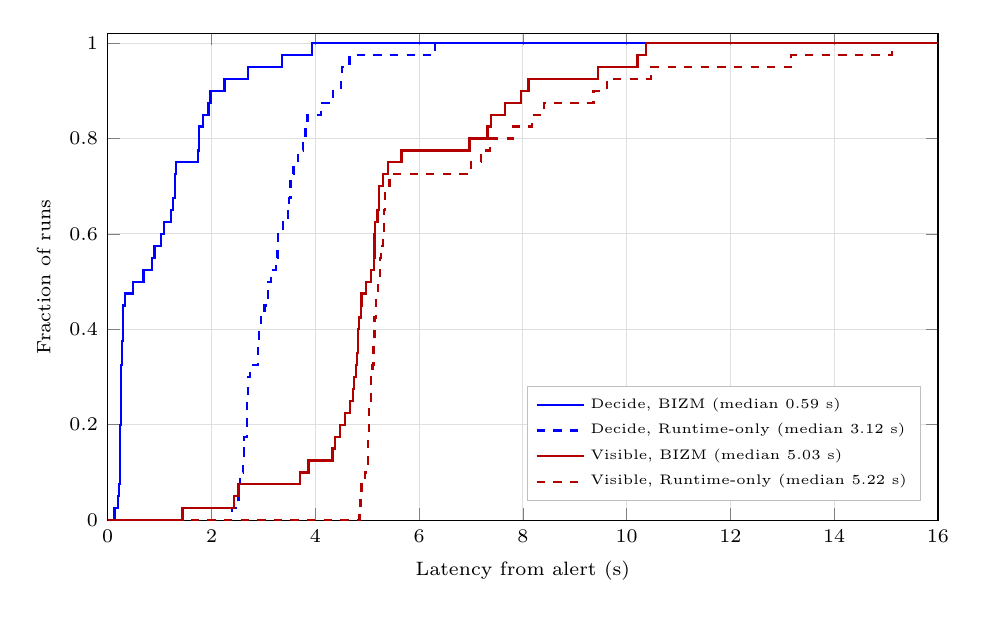
\begin{tikzpicture}
    \begin{axis}[
        width=\columnwidth, height=0.64\columnwidth,
        xlabel={Latency from alert (s)}, ylabel={Fraction of runs},
        xmin=0, xmax=16, ymin=0, ymax=1.02,
        grid=both, grid style={gray!25},
        tick label style={font=\scriptsize}, label style={font=\scriptsize},
        legend style={font=\tiny, at={(0.98,0.04)}, anchor=south east, draw=gray!50},
        legend cell align=left
    ]
    % Empirical CDFs over the 40 enforced live runs (S1 to S4) of each configuration.
    \addplot[blue, thick, const plot] coordinates {(0,0.000) (0.13,0.000) (0.13,0.025) (0.2,0.050) (0.21,0.075) (0.23,0.100) (0.23,0.125) (0.23,0.150) (0.24,0.175) (0.24,0.200) (0.25,0.225) (0.25,0.250) (0.26,0.275) (0.26,0.300) (0.26,0.325) (0.27,0.350) (0.28,0.375) (0.29,0.400) (0.29,0.425) (0.3,0.450) (0.33,0.475) (0.49,0.500) (0.69,0.525) (0.86,0.550) (0.9,0.575) (1.02,0.600) (1.09,0.625) (1.22,0.650) (1.25,0.675) (1.3,0.700) (1.3,0.725) (1.32,0.750) (1.74,0.775) (1.76,0.800) (1.76,0.825) (1.84,0.850) (1.94,0.875) (1.98,0.900) (2.25,0.925) (2.7,0.950) (3.36,0.975) (3.93,1.000) (16,1.000)};
    \addlegendentry{Decide, BIZM (median 0.59 s)}
    \addplot[blue, thick, dashed, const plot] coordinates {(0,0.000) (2.4,0.000) (2.4,0.025) (2.52,0.050) (2.53,0.075) (2.55,0.100) (2.61,0.125) (2.62,0.150) (2.63,0.175) (2.68,0.200) (2.68,0.225) (2.68,0.250) (2.71,0.275) (2.71,0.300) (2.74,0.325) (2.89,0.350) (2.9,0.375) (2.92,0.400) (2.95,0.425) (3.02,0.450) (3.09,0.475) (3.09,0.500) (3.15,0.525) (3.24,0.550) (3.27,0.575) (3.28,0.600) (3.37,0.625) (3.47,0.650) (3.5,0.675) (3.52,0.700) (3.52,0.725) (3.58,0.750) (3.66,0.775) (3.76,0.800) (3.81,0.825) (3.85,0.850) (4.11,0.875) (4.34,0.900) (4.5,0.925) (4.51,0.950) (4.66,0.975) (6.31,1.000) (16,1.000)};
    \addlegendentry{Decide, Runtime-only (median 3.12 s)}
    \addplot[red!70!black, thick, const plot] coordinates {(0,0.000) (1.44,0.000) (1.44,0.025) (2.44,0.050) (2.52,0.075) (3.71,0.100) (3.87,0.125) (4.33,0.150) (4.38,0.175) (4.47,0.200) (4.57,0.225) (4.67,0.250) (4.73,0.275) (4.75,0.300) (4.78,0.325) (4.8,0.350) (4.83,0.375) (4.83,0.400) (4.84,0.425) (4.88,0.450) (4.89,0.475) (4.97,0.500) (5.08,0.525) (5.13,0.550) (5.14,0.575) (5.14,0.600) (5.15,0.625) (5.2,0.650) (5.22,0.675) (5.22,0.700) (5.3,0.725) (5.4,0.750) (5.66,0.775) (6.97,0.800) (7.32,0.825) (7.39,0.850) (7.66,0.875) (7.96,0.900) (8.11,0.925) (9.45,0.950) (10.21,0.975) (10.37,1.000) (16,1.000)};
    \addlegendentry{Visible, BIZM (median 5.03 s)}
    \addplot[red!70!black, thick, dashed, const plot] coordinates {(0,0.000) (4.85,0.000) (4.85,0.025) (4.87,0.050) (4.89,0.075) (4.96,0.100) (5.01,0.125) (5.01,0.150) (5.01,0.175) (5.03,0.200) (5.03,0.225) (5.04,0.250) (5.08,0.275) (5.08,0.300) (5.1,0.325) (5.12,0.350) (5.12,0.375) (5.14,0.400) (5.14,0.425) (5.17,0.450) (5.17,0.475) (5.21,0.500) (5.24,0.525) (5.25,0.550) (5.26,0.575) (5.31,0.600) (5.32,0.625) (5.32,0.650) (5.35,0.675) (5.35,0.700) (5.43,0.725) (7,0.750) (7.19,0.775) (7.37,0.800) (7.81,0.825) (8.18,0.850) (8.4,0.875) (9.36,0.900) (9.62,0.925) (10.47,0.950) (13.17,0.975) (15.12,1.000) (16,1.000)};
    \addlegendentry{Visible, Runtime-only (median 5.22 s)}
    \end{axis}
    \end{tikzpicture}
    \caption{Empirical distributions of decision latency and rule-visibility latency on the live scenarios (S1 to S4, $N=40$ enforced runs per configuration).}
    \label{fig:latency_cdf}
\end{figure}

Over the 77 labeled live and S6 decisions, BIZM makes no error: precision 100\% (95\% CI [93.5, 100]), threat-containment rate 100\% [93.5, 100], false positive rate 0\% [0.0, 15.4], and accuracy 100\% [95.3, 100]. The runtime-only configuration, over 140 decisions, reaches precision 100\% [95.9, 100], TCR 98.9\% [94.0, 100] (F1 99.4\%), FPR 0\% [0.0, 7.1], and accuracy 99.3\% [96.1, 100]. Its single miss is an inbound-management case answered log-only: a DB-OLTP host opening SSH toward MGT (SID 9000011). The compiled path contains this case in all three runs, because it decides from the documented response and the denied verdict of the pair; this is the policy-verdict confirmation that the runtime path lacks. In four of its forty legitimate S6 decisions the runtime LLM proposed a DROP, which the policy-conflict check (three) and the severity gate (one) rejected before enforcement. The intervals show that these figures are evidence of feasibility on this scenario set, not a guarantee of zero errors.

The upper part of Table~\ref{tab:baselines} reports the matrix sweep. Static segmentation answers none of the 42 containment cases. Host isolation contains the most but cuts 6.3 times more legitimate flows than flow-scope containment, and it over-blocks the four protected-source cases. The synthesized program decides all 75 cases at flow scope and agrees with the runtime path and Baseline-C, which coincide with it on these single-alert cases; their differences lie in the parts of the domain the sweep does not sample (Section~\ref{sec:compiled_fidelity}). Every service edge removed falls on a permitted pair, because on a denied pair the static matrix has already removed it. Because the compiled path is deterministic, the five runs of a case are not independent; the table therefore reports intervals over the 75 distinct cases, and the exact McNemar test between host isolation and BIZM on those cases gives $p=0.125$ (four discordant cases), whereas treating the 375 decisions as the unit would give $p=1.9\times10^{-6}$. The sweep is a coverage check of the policy matrix, not a sample from traffic, and its intervals should be read as such.

\subsection{Adversarial Safety and Bounded-Isolation Guarantees (RQ5)}
\label{sec:adversarial_safety}

The upper part of Table~\ref{tab:safety} reports adversarial-safety results. Scenario S7 contains prompt-injection alerts that attempt to redirect isolation to protected control-plane addresses, low-severity alerts that attempt to bypass the severity gate, and spoofed-source cases. BIZM produces no unsafe enforcement in its 27 decisions, nor in the 90 decisions of the runtime-only configuration, which bounds the violation rate on this scenario set below 12.8\% and 4.0\% at 95\% confidence. With the synthesized program, the injected alerts never reach a model: the program decides from the alert source, zones, and signature and ignores alert text, so the injected instructions have nothing to act on. The injection cases were contained at their true source, and the spoofed-source and low-severity cases were removed by the protected-asset and severity gates. In the runtime-only configuration, the protected-asset set and off-target checks reject injected targets.

Baseline-B, which uses the same LLM without deterministic safety layers, violates safety in 100\% of its 90 adversarial decisions (95\% lower bound 96.0\%). It follows injected instructions, targets protected services, or accepts unsafe redirections. Scenario S8 stresses the protected-asset invariant directly by making management or monitoring hosts appear malicious. BIZM respects the never-block constraint in all 12 protected-host decisions and the runtime-only configuration in all 40, with 95\% lower bounds of 73.5\% and 91.2\%; both surface the events for review, whereas Baseline-B isolates protected hosts. BIZM's safety is therefore not a property of the model; it comes from deterministic validation and least-privilege enforcement around the model.

The adversarial cases are author-written, but on the compiled path two attack classes are excluded for every alert, not only the tested ones. Target-fidelity confusion cannot occur because the language has no target field, and TTL abuse cannot occur because the verifier checks the TTL bounds on every point of $D(K)$ (Proposition~\ref{prop:exhaustive}). The spoofed-source cases of S7 spoof protected addresses, which the protected-asset gate removes. Spoofing a \emph{non-protected} address is not a safety violation under the invariants: the rule that results is bounded, time-limited, and scoped to connections the spoofed address initiates toward one destination and port. It is an availability vector, and the decoy variant of S11 below measures it.

\paragraph{Coordinated multi-source campaign}
A campaign from many sources attacks a different control: the global blast-radius limit. Scenario S11 launches policy violations from $n_s$ non-protected sources within 60 seconds, in a direct variant and in a decoy variant in which the alerts are produced by spoofed non-protected addresses whose purpose is to exhaust the limits. \red{The lower part of Table~\ref{tab:safety} shows that with the default limits (five rules per minute, fifty active) BIZM contains all sources for $n_s\le 5$ and the first five within the first minute for $n_s\in\{8,12\}$, after which the per-minute limit holds further containment until the next window; all $n_s$ sources are contained within [t] seconds, and no legitimate flow is cut in any run. In the decoy variant, [d] decoy addresses consume the per-minute budget for [w] s, during which a real violation from a further source is contained only after [t'] s; the per-source cap of three rules in five minutes bounds what any single decoy can consume. Raising the per-minute limit to [L'] contains all twelve sources within the first window at the cost of [describe exposure]. This confirms the intended fail-closed behavior, under which a saturated limit delays containment rather than widening it, and quantifies the containment delay an operator trades for the limit.}

\begin{table}[t]
    \centering
    \caption{Adversarial safety on S7 and S8 (upper part) and the multi-source campaign S11 under the default blast-radius limits (lower part, \red{to be filled}; $N$ runs per $n_s$).}
    \label{tab:safety}
    \scriptsize
    \setlength{\tabcolsep}{2.5pt}
    \begin{tabular}{@{}lcccc@{}}
        \toprule
        \textbf{Metric} & \textbf{BIZM} & \textbf{RT-only} & \textbf{Baseline-B} & \\
        \midrule
        Violation rate (S7)    & 0.0\%   & 0.0\%   & 100.0\% & \\
        Availability (S7)      & 100.0\% & 100.0\% & 11.1\%  & \\
        Never-block (S8)       & 100.0\% & 100.0\% & 0.0\%   & \\
        \midrule
        \textbf{S11 ($n_s$, variant)} & \textbf{1st min} & \textbf{Total} & \textbf{Time (s)} & \textbf{FP} \\
        \midrule
        3, direct  & \tbd & \tbd & \tbd & \tbd \\
        5, direct  & \tbd & \tbd & \tbd & \tbd \\
        8, direct  & \tbd & \tbd & \tbd & \tbd \\
        12, direct & \tbd & \tbd & \tbd & \tbd \\
        12, decoy  & \tbd & \tbd & \tbd & \tbd \\
        \bottomrule
        \multicolumn{5}{@{}p{0.97\columnwidth}@{}}{\footnotesize RT-only: Runtime-only. 1st min / Total: sources contained (of $n_s$) within the first minute and in total; Time: seconds until all sources are contained; FP: legitimate flows cut.}
    \end{tabular}
\end{table}

\subsection{Residual Reasoning and Ablation Analysis (RQ6)}
\label{sec:reasoning_ablation}

The lower part of Table~\ref{tab:baselines} reports the signature-hint ablation. Scenario S9 contains malicious known-signature cases, malicious unknown-signature cases, and legitimate unknown-signature cases. In BIZM, known signatures are decided by the synthesized program and unknown signatures by the runtime path. On malicious unknown signatures, BIZM is correct in seven of nine decisions and the runtime-only configuration in 28 of 30, whereas SOAR-A is correct in none because it has no matching playbook entry. The runtime path infers maliciousness from context: source and destination zones, policy-matrix entry, connection direction, signature text, and baseline behavior. Both BIZM misses concern one case, held once at confidence 0.66 for review and answered once as log-only, so they fall on the review side rather than on enforcement. On legitimate unknown signatures, both configurations correctly choose no enforcement in all cases.

\begin{table}[t]
    \centering
    \caption{Comparison with the baselines on the matrix sweep (upper part; 75 distinct cases, each repeated 5 times with identical outcomes; SOAR-A uses host isolation) and on the S9 reasoning ablation (lower part; correct decisions). Edges and Cut are totals over the 75 distinct cases.}
    \label{tab:baselines}
    \scriptsize
    \setlength{\tabcolsep}{1.2pt}
    \begin{tabular}{@{}lccccc@{}}
        \toprule
        \textbf{Measure} & \textbf{Static} & \textbf{SOAR-A} & \textbf{Basel.-C} & \textbf{RT-only} & \textbf{BIZM} \\
        \midrule
        Sweep accuracy          & 44.0\% & 94.7\% & 100.0\% & 100.0\% & 100.0\% \\
        Edges closed            & 0 & 88 & 7 & 7 & 7 \\
        Legit.\ flows cut       & 0 & 44 & 7 & 7 & 7 \\
        \midrule
        S9 malicious, known     & n/a & 30/30 & n/a & 30/30 & 9/9 \\
        S9 malicious, unknown   & n/a & 0/30  & n/a & 28/30 & 7/9 \\
        S9 legit., unknown      & n/a & 30/30 & n/a & 30/30 & 9/9 \\
        S9 total                & n/a & 60/90 & n/a & 88/90 & 25/27 \\
        \bottomrule
        \multicolumn{6}{@{}p{0.97\columnwidth}@{}}{\footnotesize Sweep accuracy over the 75 distinct cases, 95\% Clopper-Pearson intervals: Static [32.5, 55.9]; SOAR-A [86.9, 98.5]; Baseline-C, Runtime-only, and BIZM [95.2, 100]. Basel.-C: Baseline-C; RT-only: Runtime-only.}
    \end{tabular}
\end{table}

Scenario S10 injects a three-stage campaign from one source: scanning, application-tier bypass, and database bypass. The synthesized program contains the third stage in all three sequenced and all three cold runs. The runtime-only configuration identifies the multi-stage pattern in all ten runs and cites earlier stages in its reasoning trace, while SOAR-A mitigates only the final signature-matched event. The confidence score does not increase between isolated and correlated presentations because clear violations already saturate near the top of the model's coarse confidence scale.

This ablation should be interpreted narrowly. The synthesized program covers what the knowledge base determines; the runtime path is needed where it does not, such as unknown signatures and alerts that contradict the catalog, and it is less reliable there. The safety invariants remain necessary because the same reasoning component can be wrong or manipulated.

\subsection{Algorithm Inputs and Parameter Sensitivity}
\label{sec:sensitivity}

The inputs of Algorithms~\ref{alg:synthesis} and~\ref{alg:decision} are exercised as follows: the policy $P$ (verdict and conflict check) by S1 to S3, S6, and the sweep; the baseline $B$ (permitted-path judgment) by S4, S5, and S9; the protected set $\mathcal{N}$ by S7, S8, and the sweep; the severity gate $\ell$ by S7 and RQ1; the history $H(s)$ by S10 and RQ1; the program $\Pi^{\oplus}$ by RQ1, RQ2, and the live scenarios; the synthesis parameters $k$, $\eta_{\max}$, and $T$ by RQ1 and RQ3; the confidence gates $\tau_c$ and $\tau_\Pi$ by S9 and the threshold sweep below; the TTL bounds by the S1 to S4 post-enforcement checks; and the active-rule set $\mathcal{R}$ and the blast-radius limits $\mathcal{L}$ only by S11, because no evaluated decision in S1 to S10 was rejected as a duplicate, by a blast-radius limit, or by the circuit breaker.

The confidence threshold was varied by gating the recorded confidences again: for the runtime path over the 140 runtime-only decisions, and for the compiled path over the 2,510 graded contain points of the deployed program. Raising $\tau_c$ from 0.70 to 0.85 changes nothing, because no evaluated runtime-only decision was enforced below 0.88, so the runtime-only TCR stays at 98.9\% and the compiled TCR at 100\%. Raising it to 0.90 loses the five live threats decided at 0.88, and the runtime-only TCR falls to 93.3\%; at 0.95 it falls to 2.2\%, and the compiled TCR to 0\%, because every \textsc{drop} rule of the synthesized program carries confidence 0.90, the lowest value among agreeing members, so a threshold above 0.90 requires resynthesizing the program rather than changing a configuration value. The false positive rate stays at zero at every threshold, because the four legitimate cases for which the runtime model proposed a DROP were rejected by the policy-conflict and severity checks, not by the confidence gate.

The TTL bounds do not change any reported outcome: rules became visible within ten seconds of the decision, well inside the 60-second minimum, and all post-enforcement checks passed before expiry. The blast-radius limits bound bursts above five rules per minute or three per source within five minutes, which S1 to S10 do not produce; their effect under a multi-source campaign is reported in Section~\ref{sec:adversarial_safety}.

\subsection{Overhead, Cost, and Verifier Scalability (RQ6)}
\label{sec:overhead}

A runtime decision issues one reasoning call and one audit-trace call with a mean prompt of 10.1K tokens, dominated by the retrieved context, or about 21K tokens per enforced decision. A compiled decision uses no tokens and takes 2 to 17 ms without enforcement; its decision latency on the testbed is the Secure Framework round trip. Synthesis is a one-time cost of 341K tokens and 117 seconds, about the tokens of 16 runtime decisions, repeated only when the knowledge base changes. In the injected runs, the synthesized program answered 45 of the 72 alerts that passed the gate; the runtime path answered the other 27 with a median of 23.7 seconds, against a live runtime-only median of 3.1 seconds. \red{[Not explained by the audit-trace call or by queueing: under the same injection harness, the runtime-only configuration decided its 220 injected alerts with a median of 3.4 s (95th percentile 5.5 s). The 27 runtime-path decisions of these runs are to be remeasured.]}; the 15-second timeout applies to the enforcement-facing call alone. No reported decision was served from the decision cache: every enforced runtime decision took at least 2.2 seconds, the time of a model call.

\paragraph{Throughput}
\red{Under an offered load of [$\lambda$] alerts per second of covered signatures, the compiled path sustains a decision rate of [$\mu$] alerts per second on the testbed host with a median decision time of [x] ms and no queue growth, whereas the runtime-only configuration saturates at [$\mu'$] alerts per second, limited by the model-call concurrency of [c]. Beyond that load, the runtime queue grows and the median decision latency exceeds [y] s after [z] s of sustained load.} These figures are for the decision plane alone; the enforcement path adds the gNMI round trip reported above and is not stressed by alert rate, because duplicate alerts for a covered flow are suppressed while its rule is active.

\paragraph{Verifier scalability}
By Proposition~\ref{prop:cost}, the verification cost grows linearly with $|D(K)|$, which itself grows quadratically in the number of zones and linearly in the number of signatures. For fabrics of $(|Z|,|\Sigma_K|)=(16,60)$, $(32,120)$, and $(64,250)$, the domain has 987,224, 7,379,064, and 59,386,600 points, against 136,080 for the deployed testbed, and linear scaling from the deployed measurement of 5 s projects single-core verification times of about 36 s, 271 s, and 36 min. \red{Measured times on synthetic knowledge bases of these sizes are [t$_{16}$], [t$_{32}$], and [t$_{64}$] s on a single core and [t$'_{16}$], [t$'_{32}$], and [t$'_{64}$] s with parallel evaluation across signatures on [p] cores, confirming the linear growth.} Because a synthesis with $k=5$ and $\eta_{\max}=3$ issues at most 26 verifications, even the largest listed fabric remains within an offline budget of minutes, and verification can further be restricted to the realizable sub-domain $R(K)$ when the IDS catalog fixes the severity and zone coverage of each signature.

BIZM is intended for containment rather than packet-level inline filtering; high-rate traffic mitigation is better handled by in-network or programmable data-plane mechanisms. Production deployment would also require queueing, overload thresholds, and fail-safe modes for the runtime path, which the throughput experiment characterizes only on the decision plane.

\subsection{Discussion, Limitations, and Threats to Validity}
\label{sec:discussion_validity}

The results support three conclusions. First, the LLM contributes most as a synthesizer under verification: a program it derives from the knowledge base agrees with the knowledge base on every graded point, follows its prose where a hand-written rule does not, is resynthesized when the knowledge base changes, and is admitted only after an exhaustive check that rejected three of the six initial candidates. Second, LLM-assisted response can be made operationally useful when the model is not granted direct authority over the network; on both paths, safety comes from deterministic validation and least-privilege enforcement, and on the compiled path it is established on every input in advance. Third, the evaluation provides feasibility evidence on a controlled testbed, not proof of production-scale readiness.

The main limitations are clear. Ground truth is derived from a knowledge base the authors wrote, and the four changes in RQ2 were also authored; a wrong knowledge base yields a program that is consistently wrong, although never unsafe, and the verifier checks safety invariants, not agreement with intent. The program features are coarse, so multi-hop pivot reasoning and payload evidence remain with the runtime path. The testbed is virtualized and small, the scenario set is author-designed, injected alerts do not exercise the IDS sensor, and \red{the cross-model experiment covers two open-weight models}. The model confidence is not calibrated; it saturates on clear violations, so the confidence threshold acts as a conservative floor rather than a probabilistic discriminator. The verifier is exhaustive only because the feature abstraction is finite; richer features would require a symbolic verifier, which is a direction for future work rather than a limitation of the guarantee stated here.

There are operational trade-offs. Automatic containment of high-impact assets carries operational risk, which a human-in-the-loop mode for protected assets can address. Blast-radius limits trade containment delay for bounded impact under a coordinated campaign, as S11 quantifies. Target fidelity binds the rule to the header source, so an attacker who can spoof a non-protected address can cause a bounded, time-limited denial of that address's connections to one destination and port; source-address validation at the leaf, which is orthogonal to BIZM, closes this vector, and the per-source and per-minute limits bound it where it remains open. The threat model assumes a correct enforcement implementation and does not cover compromise of the switch operating system, the IDS engine, or encrypted payload inspection beyond what the IDS can observe. \red{A knowledge-base fault-injection experiment, in which seeded errors in the catalog are propagated through synthesis, would substantiate the claim that a wrong knowledge base yields a consistently wrong but never unsafe program; it is left for the supplementary material.}

Finally, prior systems are compared by capability rather than by numerical performance (Table~\ref{tab:positioning}), because they address different stages of the loop. Baseline-C stands for deterministic context; a learned, anomaly-driven responder was not compared. Schema validation, role-based authorization, TTL-bounded rules, and protected-asset allowlists are established security-engineering mechanisms, and BIZM does not claim them as new. The contribution of BIZM is not a higher detection score but a bounded response architecture that synthesizes verified response logic from the architecture description and connects alert interpretation, safety validation, and least-privilege enforcement in one closed loop.

\section{Conclusion}
\label{sec:conclusion}

This paper presented BIZM, a safety-constrained framework for bounded isolation in Zero Trust microsegmentation that treats east-west response as a verification-guided synthesis problem. An LLM synthesizes the architecture knowledge base into a response program of a target-free language; an exhaustive verifier checks the bounded-isolation invariants on every point of the finite alert domain and guides repair with typed counterexamples; and a strict-majority ensemble of verified programs, which we prove remains verified, is deployed and bound to the knowledge base it was synthesized from. At runtime, the LLM reasons only over the alerts the program does not cover. On both paths, enforcement is restricted to source-faithful, time-bounded, provenance-marked DROP rules, and each action must pass fail-closed validation and command-level authorization before reaching the fabric, which bounds the authority of the model even when its output is mistaken, malformed, or manipulated.

The evaluation on a spine-leaf data-center testbed shows that the synthesized program agrees with the knowledge base on all 14,970 graded points, where a hand-written contextual rule reaches 96.1\%; that the verifier rejected three of the six initial candidates, which repair corrected within one round; and that resynthesis keeps 99.97\% to 100\% agreement after four knowledge-base changes. On the live testbed, BIZM contains every threat without a false positive, decides in 0.6 instead of 3.1 seconds, and produces no unsafe enforcement under the tested adversarial alerts\red{, including a coordinated multi-source campaign}. These results support the central argument of the paper: LLM-assisted microsegmentation response is feasible when the LLM synthesizes verified response logic from the architecture and its runtime authority is bounded by deterministic network-level safety invariants.

The current prototype has clear limitations. The evaluation uses a controlled virtualized fabric, an author-written knowledge base and scenario set, a coarse program feature set, and \red{two} open-weight models. Future work will extend the program features toward multi-hop context with a symbolic verifier, evaluate on larger and more diverse traffic, synthesize from operator-maintained documentation, and develop human-in-the-loop policies for high-impact protected assets and management-plane events.

\section*{Declaration of Competing Interest}
\noindent The authors declare that they have no known competing financial interests or personal relationships that could have appeared to influence the work reported in this paper.

\section*{Funding}
This work was supported by the Ministry of Science and Technology of Vietnam under the National Science and Technology Program, project code KC.01.06/21-30.

\section*{Data and Code Availability}
The testbed configuration, Suricata rules, policy matrix, knowledge base, response-language definition, verifier, synthesis prompts, decision schemas, scenario definitions, and evaluation scripts will be made available upon publication to support reproducibility. An anonymized supplementary package can be provided for review upon request.

\section*{Declaration of Generative AI and AI-Assisted Technologies in the Writing Process}
During the preparation of this work, the authors used generative AI and AI-assisted technologies to refine the scientific prose, improve readability, and polish LaTeX formatting. After using these technologies, the authors thoroughly reviewed and edited the content as needed and take full responsibility for the content of the published article.

\section*{CRediT Authorship Contribution Statement}
\textbf{Hanh P. Du}: Conceptualization, Formal analysis, Investigation, Methodology, Validation, Writing (original draft).
\noindent \textbf{Hung K. Luu}: Writing (original draft), Writing (review \& editing), Visualization, Validation, Software, Investigation, Formal analysis.
\textbf{Minh T. Nguyen}: Visualization, Validation, Software, Investigation, Formal analysis, Writing (original draft).
\textbf{Hoa N. Nguyen}: Writing (original draft), Writing (review \& editing), Methodology, Conceptualization, Project administration, Supervision.

\balance
\bibliographystyle{elsarticle-num}
\bibliography{refs}

\end{document}